\documentclass[12pt,a4paper]{article}


\usepackage[a4paper, margin = 1.25in]{geometry}


\usepackage{natbib} % for bibliography Chicago style
\usepackage{amsmath} % for math symbols
\usepackage{amssymb} % some more math symbols
\usepackage{graphicx}  % to attach graphics
\usepackage{epstopdf}
\usepackage[font=small]{caption} % to caption graphics
\usepackage{booktabs} 
\usepackage{bm}
\usepackage{listings}
\usepackage{array} % package to center entries in table
\usepackage[utf8]{inputenc} 
\usepackage[english]{babel}
\usepackage{titling} % Package for separated title page environment
\usepackage{multirow} % package for tables
\usepackage{lscape} % for setting up landscape table and figures
\usepackage{tikz}


\newcolumntype{P}[1]{>{\centering\arraybackslash}p{#1}} % to center entries in table
\newcolumntype{M}[1]{>{\centering\arraybackslash}m{#1}} % Vertical centering
\setlength{\parskip}{1em}
\newcommand{\forceindent}{\leavevmode{\parindent=2em\indent}} % force indent custom function
% \renewcommand{\thefigure}{\arabic{section}.\arabic{figure}} % Redefine the figure numbering
% \renewcommand{\thetable}{\arabic{section}.\arabic{figure}} % Redefine the table numbering
\DeclareMathOperator*{\argmin}{arg\,min} % Define argmin in math mode
\DeclareMathOperator*{\sgn}{sgn} % Define sgn() in math mode
\newtheorem{theorem}{Theorem} % Declare theorem environment
\newtheorem{definition}{Definition} % Declare theorem environment


\graphicspath{ {./graphic/} }
\title{LASSO-based predictive regression for stock returns \\~\\
\large Master's thesis \\
\large for the Master's degree programme Economics in the Faculty of Business, Economics and Social Sciences at the Christian-Albrechts-Universität zu Kiel \\~\\
\large Submitted by \\~\\
\large Hieu, Hoang}
\date{}

\begin{document}
\pagenumbering{gobble} % this is to supress numbering
\begin{titlepage}
	\maketitle
	\mbox{} \\[1in]
	First assessor: Prof. Dr. Matei Demetrescu \\
	Second assessor: Prof. Dr. Kai Carstensen \\
	Kiel, January, 2020
	
\end{titlepage}

\section*{Table of Contents}
\pagenumbering{arabic} % Restart numbering
\tableofcontents
\newpage

\section{Introduction}
Prediction of stock returns has always been an important subject in finance, since an accurate prediction can help investors decide the portions of safe and risky assets in their portfolios, generating optimal wealth for their clients and themselves. As a result, a large volume of literature has been dedicated to developing asset pricing theory and predictive statistical models. One of the most popular and long-standing bases in the realm of asset pricing is the efficient market hypothesis (EMH), summarized and popularized in \cite{fama1970efficient}. According to EMH, equity premium is constant and reflects all available information. Hence, market anomalies and historical average of premia are analyzed to forecast asset returns.

On the other hand, financial econometricians focus on including relevant lagged financial and macroeconomic variables as predictors for equity premium as a way to exploit market inefficiency. \cite{fama1988dividend}, \cite{schiller1998valuation}, among others explored the power of using valuation ratios, e.g. dividend-price ratio, dividend yield, earnings-price, book-to-market ratio to forecast long-term returns of stock, while \cite{fama1990stock}, \cite{schwert1990stock}, and related papers showed correlation between bonds (treasury and corporate) and stock returns. As a result, a healthy number of literature demonstrated and cemented this idea, see, among \cite{hodrick1992dividend}, \cite{kothari1997book}, \cite{lamont1998earnings}, 
\cite{pontiff1998book}.

As of the late 1990s and early 2000s, the common consensus within the field is that excess stock returns can be predicted \citep{welch2008comprehensive}. However, along with new tools come new challenges. One of which is that the results of aforementioned findings may very well be spurious. \citep{stambaugh1999predictive} showed that when the innovation of a predictor is correlated with excess return, which is the case for many valuation ratios, the resulting estimated coefficient is biased and exhibits sharply different finite-sample properties from the standard case. One apparent example is the dividend yield which has the same return component with equity premium. A second source for spurious result stems from the high persistence of predictors. It has been well-known that a regression model with integrated or near-integrated predictors may sometimes produce 'non-sense correlation' where highly significant betas and high R-squared values are obtained while no "real" and meaningful correlation exists, except for the case of co-integrated series; see among \cite{yule1926we}, \cite{granger1974spurious}, \cite{phillips1986understanding}, \cite{granger2001spurious}, and \cite{engle1987co}. Last but not least, the problem of near-collinear predictors is also apparent for financial econometricians. As stated above, many highly persistent time series variables exhibit meaningless high cross-correlation scenario, but high correlation nonetheless. Furthermore, some ratios are by construction derived from other ratios or macroeconomic variables, hence the possible long-term co-movement between said ratios. This in turn causes the design matrix to become nearly singular (asymptotically singular), which produce estimation inconsistencies and failures in central limit theory in least square regression even in the case of stationary predictors and strong regression signal \citep{phillips2016inference}, much less for our case of high-persistence.

For the reasons stated above, OLS may not be the best way to go. The late 1990s and early 2000s also witnessed a relatively new method for estimating linear models: the lasso \citep{tibshirani1996regression}. Instead of just minimizing the residual sum of squares, the lasso further applies a constraint to the sum of absolute values of estimated coefficients. This penalty term helps shrink coefficient estimates and at the same time encourages some variables to take on zero as coefficient, effectively eliminate them from the model. Thus, the lasso has the advantages of both (continuous) model selection and variance reduction by trading off some amount of bias, which may increase predictive performance. Belonging to the penalized least squared family of regression method, lasso also benefits from stability when there exists high collinearity between predictors by preventing coefficient inflation as in the case of its brother shrinkage variation, the ridge regression. Still, lasso suffers from a number of problems, mainly related to inference. Additionally, we still have the problem of near-singular design matrix and near-integrated and integrated series, potentially cointegrated in our hand.

This paper will be organized as followed. This section gave an introduction to the paper. Next, I will review some literature regarding the problem of asymptotically degenerate design matrix, and how it makes OLS estimations invalid. An overview of lasso (and its variants) and how lasso can be used to combat our prevailing problems will also be discussed in this section. The third section will be about the technical details of Adaptive Lasso (henceforth alasso), with focus on the inference of coefficient estimates. The fourth section compares predictive performance of alasso with regular lasso, autoregressive of order 1, and OLS in simulation settings. Lastly, I will apply alasso to Goyal's data set used in \cite{welch2008comprehensive}, with updates until 2018, to assess its real-world predictive performance. Conclusion and extension will be given as closing thoughts.


\section{Literature Review}
In this section, I will first review a number of the literature that discusses our three big problems in the context of OLS regression: correlation between innovation of lagged predictor and regression disturbance; mixed roots, high persistence predictors; and near-singular design matrix. Next, we will take a look at how lasso-type regression, specifically alasso, can help alleviate parts of our problems.

OLS, or ordinary least squares, is a long-standing powerhouse in the scene of linear regression. The objective of OLS is to find a set of coefficients that minimizes the squared differences between observed dependent variables and its predicted value. Thank to its readily available analytical solution, fast computation, and well-studied inference, it is widely used in both cross-sectional and time series data alike. However, there are a set of assumptions required to make the OLS estimates valid. Specifically, the stochastic processes involved must be stationary and ergodic, and disturbances need to be uncorrelated to the regressors. However, evidences for stationarity of valuation ratios are mixed and shaky, and endogeneity problem looms large. \cite{roll2002rational} argues that under rational expectation, asset price is non-stationary due to its dependence on expectation of future quantities. Yet, metrics that are constructed as functions of price, e.g market-to-book, earning-price ratios, dividend yields,... may exhibit different root characteristics \citep{phillips2015halbert}. At the same time, most remaining series show high yet imprecisely determined degree of persistence, leading to the problem of mixed roots, possibly cointegrated, regression; and nonstationarity leads to the endogeneity effect in the limit, leading to non-standard limit theory \citep{phillips2015halbert}. The same paper also discusses 'misbalancing' issue, where predicted variable and predictors have different memory types. The solution out is not straight-forward. \cite{elliott1994inference} discussed two common simple solutions: ignore the problem altogether, or determine the post-regression inference by pretesting predictors for unit roots. Both lead to the substantial over-rejection of the null of no significance. The solution proposed in the same paper involves Bayesian statistic, thus may not be appealing to some. In another approach, a local-to-unity autoregressive specification in the form of $ \rho = 1 + \frac{c}{n} $ is used to conduct asymptotic theory. However, the introduction of the unknown parameter brings more issues. Since localizing coefficient $c$ is not consistently estimable, asymptotic bias cannot be corrected, leading to nonstandard limit theory. \cite{phillips2013predictive} discussed $c$ and suggested possible solutions.

Another violation of OLS assumptions comes in the form of high to perfect correlation between predictors. In the case of perfect correlation, removing inappropriate regressor(s) is a common remedy. When the correlation is not perfect, determinant(s) of design matrix gets into the vicinity of zero, causing computational difficulty in matrix inversion and inflated coefficient estimates. However, removal of regressors is not always an preferable option since each regressor may contain some additional information that can improve the model fit or prediction. In the case of predicting excess returns, some predictors may contain information about market inefficiency despite high correlation due to a common variable in their construction. This kind of construction also leads to possible co-movement of predictors, causing singularity in the limit (near-singular design matrix). As variable frequency increases such as in the case of financial data, singularity can come very quickly.

In this paper, I would like to introduce a relatively new method of estimation for linear model that has the ability to hopefully overcome some of the aforementioned issues. Proposed and discussed by \cite{tibshirani1996regression}, the lasso (least absolute shrinkage and selection operator) exhibits some more preferable properties than the well-known OLS.

First, while shrinking coefficients introduces some amount of bias, it helps to prevent estimate inflation in presence of high-collinearity. In fact, for the case of near-singular design, the lasso estimates are consistent, and with an appropriate choice for shrinkage parameter $ \lambda $, limiting distribution is normal \citep{knight2000asymptotics, knight2008shrinkage}. This result is especially handy for the case in this paper.

Second, lasso can set some coefficients to zero, effectively performs continuous model selection. Via this mechanism, variance is reduced and hence accuracy may increase in the case of predictive regression. Continuous model selection has some advantages over discrete model selection, for example subset selection, where small change in data can lead to substantially different selection outcome, or be trapped in a local optimum \citep{breiman1995better}. Furthermore, as the number of regressors increases, discrete selection is computationally hard. On the other hand, continuous selection process is more stable, intepretable, and can scale easily with a large number of variables \citep{tibshirani1996regression}. However, plain-vanilla lasso is not always consistent in identifying the right subset of variables, and does not always exhibit 'oracle properties' (consistency in variable selection and asymptotic normality) \citep{meinshausen2004consistent, zou2006adaptive}. Hence, the Adaptive Lasso (alasso) is proposed by \cite{zou2006adaptive}. Alasso assigns weights to each coefficients, and if the weights are cleverly chosen and data-driven, alasso can enjoys oracle properties. 

Last but not least, the alasso works well in the case of mixed degree of persistence in predictive regression mentioned above. It can even adapt to system of predictors that exhibits cointegration by assigning appropriate penalty level inside the system without knowing the identity of these predictors. \cite{lee2018lasso} establish and demonstrate a simple condition on $\lambda$ that leads alasso to oracle properties without knowledge of persistence level in advance.

With all the favorable theory at hand, we will embark on testing the performance of alasso in both simulation and real data settings. But first, I will re-establish important results mentioned above in a more concrete manner.

\section{The Adaptive Lasso and Its Advantages}
In this section, we will discuss the advantage of alasso. The theoretical framework will closely follow \cite{tibshirani1996regression, knight2008shrinkage, zou2006adaptive, lee2018lasso}. The proof for theorems and theoretical results are not given here, and can be found in referenced papers/articles. 

\textbf{THE MODEL}
The linear model is assumed to be as following, adapted from \cite{lee2018lasso}: \begin{equation}\label{eq:1}
\begin{aligned}
	y_i & = \sum_{l=1}^{p_z}z_{il}\alpha_{l}^{*} + 
	\sum_{l=1}^{p_x}x_{il}\beta_{l}^{*} + 
	\sum_{l=1}^{p_c}x_{il}^c\phi_{l}^{*} +
	\varepsilon_i \\
		& = \bm{z}_i'\alpha^* + 
		\bm{x}_i'\beta^* + 
		\bm{x}_i'^c\phi^* + \varepsilon_i \\
		& = \bm{w_i}'\bm{\theta} + \varepsilon_i, \\
	\bm{y} & = \bm{w}'\bm{\theta} + \bm{\varepsilon}.
\end{aligned}
\end{equation}
for $ i = 1,\ldots, n, $ where $ \bm{z}_i = (z_{i1}, \ldots, z_{ip_z})' $, $ \bm{x}^c_i = (x^c_{i1}, \ldots, x^c_{ip_z})' $, and $ \bm{x}_i = (x_{i1}, \ldots, x_{ip_x})' $ represent the stationary, cointegrated, and unit root regressors, respectively, and $p = p_z + p_c + p_x$ is the total number of regressors in the model. $\bm{w_i}$ is $ p \times 1 $ vector of all regressors; $\bm{\theta}$ is $p \times 1$  vector of all coefficients; and $ \bm{w} $, $ \bm{y} $, $ \bm{\varepsilon} $ are the observation-stacked vectors/matrices.  The presence of heterogeneous degrees of persistence and cointegration in our regressors nicely follows practical situation in predicting excess return with multiple valuation ratios and macroeconomic variables.

One deviation from the model laid out in \cite{lee2018lasso} is that regressors are allowed to have increasingly strong correlation between one another. Specifically, as sample size $ n $ increases, the degree of correlation between said regressors also increases and approaches 1. This setting is included to emulate near-singular design matrix phenomenon frequently encountered in stock return predictive regression. Later, we will see that the sequence of tuning parameter $ \lambda $ proposed by \cite{lee2018lasso} intended for mixed root in regressors is also helpful in combating near-singular design. Formally, define matrix $ \bm{C}_n $ as in \cite{knight2008shrinkage}:
\begin{equation}\label{eq:2}
	\bm{C}_n = \frac{1}{n}\sum_{i = 1}^{n}\bm{w}_i \bm{w}_i'
\end{equation}
that is nonsingular for each $ n $ except for when $ n \rightarrow \infty $, then 
\begin{equation}\label{eq:3}
	\bm{C}_n \rightarrow \bm{C},
\end{equation}
where $ \bm{C} $ is singular. In practice, near-singular design can be detected by checking whether the smallest eigenvalue of $ \bm{C}_n $ is small in comparison to its trace. 
For some sequence $ \{a_n\}$ tending to infinity, assume that
\begin{equation}\label{eq:4}
	a_n(\bm{C}_n - \bm{C}) \rightarrow D_0
\end{equation}
where $ \bm{D}_0 $ is positive definite on the null space of $ \bm{C} $, that is $ \bm{v}'\bm{D}_0\bm{v} > 0 $ for non-zero $ \bm{v} $ with $ \bm{C}\bm{v} = 0 $.
Another assumption is that near-singularity affect all regressors in our model.

To ensure stationarity of $ y_i $, the effect of non-stationary regressors (including unit root components in cointegrated ones) are kept small using local-to-zero coefficients. This type of coefficient design is also useful to model the weak signal-to-noise ratio in predictive regression \citep{phillips2013predictive, lee2018lasso}. The $ p \times 1$ true coefficient $ \theta^*_n = (\theta^*_{jn} = \theta^{0*}_j/n^{\delta_j})^p_{j = 1} $ where $ \theta^{0*}_j \in \mathbb{R} $ is a fixed constant independent of sample size, and $ \delta_j \in [0, 1) $. In cases where $ \theta^{0*}_j = 0 $,  $ \delta_j $ is also set to zero. $ \theta^*_n $ thus gets smaller with increasing sample size for $ \theta^{0*}_j \neq 0 $ and $ \delta_j \in (0, 1) $, and approach zero as $ n $ tends to infinity.

On the front of identification, assumptions about error terms must also be made. While correlation between regression error and the innovation of non-stationary regressors $ \bm{x}_i $ is allowed, correlation between regression errors and innovation of stationary and cointegrated regressors is excluded (see \textbf{Assumption 3.1} and \textbf{Remark 3.1}, \cite{lee2018lasso}).


\textbf{THE LASSO}
Lasso is a technique for estimation of linear models that utilize regularization in order to shrink coefficients and perform variable selection at the same time \citep{tibshirani1996regression}. Lasso objective function for model \eqref{eq:1} are defined to be
\begin{equation}\label{eq:5}
	% \bm{\hat{\theta}}_{lasso} = 
	% \underset{\bm{\theta \in \mathbb{R}^p}}{\argmin}
	\sum_{i = 1}^n(y_i - \bm{w}_i'\bm{\theta})^2 + 
	\lambda_n\sum_{j = 1}^p\vert\theta_j\vert,
\end{equation}
which is essentially least square with an additional $ \ell1 $ penalty that helps force estimates of "small" parameter towards zero. Despite of course introducing some bias into the estimates, lasso may reduce estimation variance. In the limit, truly "small" parameters are zero with probability tends to 1 while all others are discernibly not zero. Therefore, in cases where true parameters are zero, no biases are produced and variance is reduced, a win-win situation (superefficiency, as termed in \cite{knight2008shrinkage}). On the other hand, such regularization causes bias in estimates for non-zero true coefficients while typically does not improve estimation variance considerably. Naturally, we want estimators that achieve superefficiency when $ \theta^*_j = 0 $ and produce no asymptotic bias otherwise. Studying how estimators behave in the limit regarding the choice of tuning parameter $ \lambda $ is hence a great way to come up with a desirable one. 
\cite{knight2000asymptotics} find that if $ \lambda $ is treated as a sequence dependent on sample size, and design matrix is non-singular, $ O(n) $ growth rate of $ \{\lambda_n\} $ is sufficient to obtain $ \sqrt{n} $-consistency and non-degenerate limiting distribution. However, in this paper we are more interested in cases where the design matrix is near-singular.

\textbf{NEAR-SINGULAR DESIGN MATRIX}
Assume model \eqref{eq:1} with $ \bm{C}_n $ satisfies \eqref{eq:2}, \eqref{eq:3}, and \eqref{eq:4}, that $ C $ is singular and $ D_0 $ is positive definite in the null space of $ \bm{C} $. Define $ b_n = (n/a_n)^{1/2} $ for $ \{a_n\} $ satisfies \eqref{eq:4}, and define $ Z_n $ to be
\begin{equation}\label{eq:6}
	Z_n(\bm{u}) = 
	\sum_{i = 1}^n[(\varepsilon_i - \bm{u}'\bm{w}_i/b_n)^2 - \varepsilon_i^2] +
	\lambda_n\sum_{j = 1}^{p}(\vert\theta_j + u_j/b_n\vert - \vert\theta_j\vert).
\end{equation}
This equation is a rescaled version of the objective function in \eqref{eq:5} with constants subtracted so that convergence is ensured. If $ \hat{\bm{\theta}} $ minimizes \eqref{eq:5} then $ b_n(\hat{\bm{\theta}} - \bm{\theta}) $ minimizes \eqref{eq:6}. The following theorem is adapted from \cite{knight2000asymptotics}:

\begin{theorem} [adapted from Theorem 1, \cite{knight2008shrinkage}]
	Define $ \bm{\Omega} $ to be a zero mean multivariate normal random vector such that {\normalfont Var}$ (\bm{u}'\bm{\Omega}) = \sigma^2\bm{u}'\bm{D}_0\bm{u} $ positive for each nonzero $ \bm{u} $ that satisfies $ \bm{C}\bm{u} = \bm{0} $. Let $ \hat{\bm{\theta}}_n $ minimizes \eqref{eq:5} for $ \lambda_n \geq 0$. If $ \lambda_n/b_n \rightarrow \lambda_0 \geq 0 $ then
	\[
	b_n(\hat{\bm{\theta}}_n - \bm{\theta}) \overset{d}{\longrightarrow} 
	\argmin\{Z(\bm{u}):\bm{C}\bm{u} = \bm{0}\},
	\] where \[
	Z(\bm{u}) = -2\bm{u}'\bm{W} + \bm{u}'D_0\bm{u} +
	\lambda_0\sum_{j = 1}^p\{u_j\sgn(\theta_j) + \vert u_j\vert I(\theta_j = 0)\}.
	\]
\end{theorem}
Theorem 1 reveals many interesting insights. With a proper choice of $ \{\lambda_n\} $, that is the sequence converges to a finite non-negative value $ \lambda_0 $, lasso estimate has normal limiting distribution. In the case of $ \lambda_0 = 0 $, lasso, somewhat trivially, is consistent and has the same limiting distribution as the OLS does since the penalty term vanishes. Less trivial is the case where $ \lambda_0 $ takes on positive value. Suppose all true parameters $ \theta_1, \ldots, \theta_p $ are non-zero, lasso estimate is biased, and the amount of bias depends on the vector $ \bm{u} $ and the signs of each element in the vector of true parameter $ \bm{\theta} $. By assumption in Theorem 1, the null space of $ \bm{C} $ is the space of vectors $ \bm{u} $ with $ u_1 + \ldots + u_p = 0 $, therefore $ {\normalfont Bias}(\hat{\bm{\theta}}_n) = 0 $ if true parameters all have the same sign. In another example case where $ \theta_1 \neq 0 $ and $ \theta_2 = \ldots = \theta_p = 0 $, the joint limiting distribution of $ b_n(\hat{\bm{\theta}}_{nj} - \bm{\theta}_j) $ for $ p = 2, \ldots, p $ will have positive probability mass at $ \bm{0} $. Since the limiting distribution lies in the null space of $ \bm{C} $ as in \eqref{eq:4}, $ b_n(\hat{\theta}_{n1} - \theta_1) $ is implied to have positive probability mass at 0 \citep{knight2008shrinkage}. This indicates possible asymptotic bias in the estimates of non-zero parameters. Another downside of singularity in the limit is the slower convergence rate of estimates to their limiting distributions due to $ a_n \rightarrow \infty $ and $ b_n = (n/a_n)^{1/2} $ hence $ b_n $ is only of $ o(\sqrt{n}) $. The exact margin however, still depends strongly on the growth rate of $ a_n $. 

\textbf{MIXED ROOT} Aside from near-singular design matrix, unknown degree of persistence also poses problems for not only OLS, but also for lasso. In the presence of possible unit roots (exact roots are unknown) in regressors, OLS estimates is bias in the limit due to serial dependence in the innovations. With lasso, the variable screening effect is very sensitive to the choice of tuning parameter, and each set of regressors is affected differently (\textbf{Corollary 3.7} and \textbf{Remark 3.8}, \cite{lee2018lasso}). As expected, when $ \lambda_0 = 0 $, lasso's limiting distribution collides with that of OLS since no selection takes place anymore. More interesting are cases where $ \lambda_0 \neq 0 $. For $ \lambda_0 \in (0, \infty) $, only the set of stationary receives selection. In this setting, $ \lambda_0 $ is still too small to have an effect on non-stationary part. Choosing the sequence to growth even faster, where  $ \lambda_n/\sqrt{n} \rightarrow \infty $ and $ \lambda_n/n \rightarrow 0 $, drags down convergence rate of estimates for the stationary set while still does not hit non-stationary set. Raising growth rate further however starts to introduce inconsistency (\textbf{Lemma 3}, \cite{zou2006adaptive}). As a result, it is impossible for lasso to have at the same time both variable screening and consistent estimation due to lasso having a single penalty for all $ I(0) $ and $ I(1) $ regressors.

\textbf{ADAPTIVE LASSO} Introduced by \cite{zou2006adaptive}, alasso is designed to overcome possible inconsistencies in variable selection of lasso. Alasso involves applying individual weight to the tuning parameter of each regressor. The objective function of alasso is defined as:
\begin{equation}\label{eq:7}
	% \bm{\hat{\theta}}_{alasso} = 
	% \underset{\bm{\theta \in \mathbb{R}^p}}{\argmin}
	\sum_{i = 1}^n(y_i - \bm{w}_i'\bm{\theta})^2 + 
	\lambda_n\sum_{j = 1}^p \hat{\tau}_j \vert\theta_j\vert,
\end{equation}
where $ \hat{\tau}_j = \vert\hat{\beta}_j\vert^{-\gamma} $ is the individual weight for the corresponding regressor $ j $, with $ \hat{\beta}_j $ denoting estimate from another regression method. Popular choices for $ \hat{\beta}_j $ include estimates from OLS, ridge regression, or even lasso. $ \gamma $ is a hyperparameter that is, in practice, chosen such that $ \gamma \geq 1 $ to prevent non-convex optimization problem \citep{lee2018lasso}. One can also use cross-validation to optimize for $ \gamma $. The solution for this objective function is a vector of alasso estimators $ \hat{\bm{\theta}}^{al} $.

The choice of the vector of weights $ \hat{\bm{\tau}} $ is an important aspect of alasso implementation. Usually, a data driven method such as estimates from another regression scheme is used to obtain $ \hat{\bm{\beta}}$. In our case, we will consider using estimates from OLS and ridge regression due to some favorable properties. First is the OLS, $ \hat{\tau}_j = \vert\hat{\beta}_j^{ols}\vert^{-\gamma} $. In the case of mixed roots, there is an asymptotic bias in the limiting distribution of estimates due to serial dependence in the innovations since we allow for correlation between regression error and the innovation of non-stationary regressors. Still, OLS estimates still converge at the same rate as in the case of stationary regression. For zero true coefficient, $ \hat{\tau}_j $ is also small, putting a heavier penalty on its estimate. On the other hand, the weight for non-zero estimate will converge to a small value, putting less weights on its estimate. In singular settings, however, calculating weights using OLS fails due to the elimination or false inflation of estimates for highly correlated variables. Weight using estimate from ridge regression is a good replacement. By setting lambda value close to zero, ridge estimate is argued to be a reasonable approximation for OLS estimate \citep{knight2000asymptotics}.

Under the aforementioned choice of weight vector, Theorem 1 can be extended to alasso \citep{knight2000asymptotics}. Furthermore, for $\lambda_n \rightarrow \infty $, alasso estimator achieve (asymptotical) 'oracle properties' for $ \lambda_n/\sqrt{n} \rightarrow 0 $ and $ \lambda_nn^{(\gamma - 1)/2} $ \citep{zou2006adaptive}, which means the alasso estimator
\begin{itemize}
	\item identifies the right subset model: $ P(\hat{M}_n = M^*) \rightarrow 1 $
	\item has the optimal estimation rate, $\sqrt{n}(\hat{\bm{\theta}}^{al} - \hat{\bm{\theta}}^*) \rightarrow N(\bm{0}, \bm{\Sigma}^*) $  where $ \bm{\Sigma}^* $ is the covariance matrix knowing the true subset model.
\end{itemize}
Here, $ M^* = \left\lbrace j \in \{1, \ldots, p\}: \theta^*_j \neq 0 \right\rbrace $ is the set of regressors with true-large coefficients, $ \hat{M}_n = \left\lbrace j \in \{i, \ldots, p\}:\hat{\theta}_j \neq 0 \right\rbrace $ is the set of regressors with non-zero estimates (selected regressors). As straightforward as it sounds, the case in our hand here is a bit more complicated. In the presence of mixed roots, the oracle properties for alasso estimate still exist, albeit with different conditions on $ \lambda_n $. \cite{lee2018lasso} deal with this in Theorem 3.4. The optimal $ \lambda_n $ is such that $ \lambda_n \rightarrow \infty $ and
\begin{equation}\label{eq:8}
	\frac{\lambda_n}{n^{(1 / 2) \wedge (1 - \gamma.\bar{\delta})}} + 
	\frac{1}{\lambda_nn^{(\gamma - 1)/2}} \rightarrow 0,
\end{equation} 
where the wedge denotes the minimum operator, and $ \bar{\delta} = max_{j \leq p}\delta_j $.  In practice, $ \gamma \geq 1 $ is usually chosen to ensure convex optimization for alasso implementation. With this optimal rate, consistent model selection is achieved, and rate of convergence is $ \sqrt{n} $, which is optimal, for estimates of stationary set, and $ n $ for that of non-stationary set. Set $ \gamma = 1 $, $ \hat{\delta} = 1/2 $, and use the usual formulation $ \lambda_n = c_\lambda b_n n^{1/2} $, the restriction \eqref{eq:8} turns out to be
	\begin{equation}\label{eq:9}
	c_\lambda b_n + \frac{1}{c_\lambda b_n n^{1/2}} \rightarrow 0,
	\end{equation}
where $ c_\lambda $ is a constant. Any slowly shrinking sequence such as $ b_n = (\log \log n)^{- 1} $ fulfills this restriction. However, there exists asymptotic bias in the limiting distribution of true-large non-stationary parameters while estimates for true-zero parameters and true-large parameters for stationary regressors are consistent. On the other hand, the problem of near-singularity in the design matrix still needs to be addressed. The asymptotic theory developed by \cite{knight2008shrinkage} and explored above is also applicable to alasso, as it allows for different lambda sequence for each estimate. Specifically, to deal with condition \eqref{eq:2}, \eqref{eq:3}, \eqref{eq:4}, more stringent conditions must be put to slow the growth rate of $ \lambda_n $, similar to the explored lasso case. That is, estimates for stationary regressors' true-large parameters are no longer $ \sqrt{n} $-consistent, and slower than $ n $ for the non-stationary case due to the sequence $ b_n = o(\sqrt{n}) $. Additionally, singular $ \bm{C} $ causes further possible bias in the limit of the estimates for all true-large parameters while keeping estimates for true-zero parameters unbiased. Here, I propose a more slowly growing sequence of lambda. Keeping the same construction of $ \lambda_n $ as above, set $ b_n =  1 / log(n)^\kappa $, with $ \kappa \geq 1 $. The reason for a slower growth rate of $ \lambda $ is to not too far exceed the convergence rate of OLS estimators used as weights. In the context of mixed roots, and near-singular design, OLS estimates are generally biased except for estimates for true-large stationary regressors' parameters, and the convergence rate is slower than non-singular design case. Therefore, $ \lambda_n $ for alasso needs not to grow too fast, or else the sequence will dominate convergence of the weight sequence, forcing all estimates toward zero.

\textbf{EXACT POST-SELECTION INFERENCE} On the front of post-selection inference for regularization least square, the prospect is not bright. Recently, \cite{lee2016exact} derive a way to compute exact confidence interval for lasso estimators, and also make a package for application in R. However, the results are not applicable to the case at hand here due to the now-familiar problems of mixed persistence and singularity in the limit of design matrix.

In the next section, I will present simulation results to test if the ideas presented in Section 3 has any merit.


\section{Simulation study}
In this section, the performance of lasso and alasso will be assessed by means of one-step-ahead mean squared forecasting error and variable screening rate. The scheme will followed closely Section 4 of \cite{lee2018lasso}, albeit with different specifications for data generating process.

\textbf{DATA GENERATING PROCESS} To emulate both problems we have discussed in previous Section, we set up the DGP as followed. The dependent variable $ y_i $ is generated by the process
	\[ y_i = \gamma^* + \sum^2_{j = 1}z_{ij}\alpha_j^* + 
	\sum^3_{j = 1}x_{ij}\beta^*_j +
	\sum^4_{j = 1}x^c_{ij}\phi^*_{ij} +
	u_j, \]
where $ \gamma^* = 0.3 $ and $ \theta^* = (\alpha^*, \beta^*_n, \phi^*_n) = (0, 0.3, 0, - 0.4, \frac{1}{\sqrt{n}}, 0.2, - 0.2, 0, 0) $. $ z_{i1} $ and $ z_{i2} $ follow two stationary AR(1) regressors with the same autoregressive coefficients $ \rho_{z1} = \rho_{z2} = 0.6 $. Their error terms exhibit increasing dependency, and are generated from a bivariate normal distribution $ MN(\bm{0}, \bm{\Sigma}_n) $ where $ \bm{\Sigma}_n =
 		\begin{pmatrix}
 			1 		& \rho_n \\
 			\rho_n 	& 1
 		\end{pmatrix}$, and $ \rho_n = \frac{n}{n + 1} \frac{1 - \rho_{z1}\rho_{z2}}{\sqrt{(1 - \rho_{z1} ^ 2)(1 - \rho_{z2} ^ 2)}} $. This construction of $ \bm{\Sigma}_n $ allows for increasingly large correlation between two processes $ z_{i1} $ and $ z_{i2} $, and the correlation approaches unity as $ n \rightarrow \infty $. $ x_{i1}, x_{i2} $, and $ x_{i3} $ follow three independent AR(1) processes, with the respective coefficients of (- 0.98, 0.4, 1). This is to emulate mixed degrees of persistence in our later real-world example. Lastly, $ \bm{X}^c_i \in \mathbb{R}^4 $ is an I(1) process with cointegration rank 2 based on the VECM, $ \Delta \bm{X}^c_i = \Gamma'\Lambda X^c_{i - 1} + \bm{e}_i $, where the cointegrating matrix $ \Lambda = \begin{pmatrix}
 			1 & - 1 & 0 & 0 \\
 			0 & 0 & 1 & -1
 		\end{pmatrix} $ and the loading matrix $ \Gamma = 
 		\begin{pmatrix}
 			0 & 1 & 0 & 0 \\
 			0 & 0 & 0 & 1
 		\end{pmatrix} $. In the error term $ \bm{e}_i = (e_{i1}, e_{i2}, e_{i3}, e_{i4})' $, we set $ e_{i2} = e_{i1} + \nu_{1i} $ and $ e_{i4} = e_{i3} + \nu_{2i} $ where $ \nu_{1i} $ and $ \nu_{2i} $ are independent AR(1) processes with the AR(1) coefficients (0.2, 0.4).
 
\textbf{BENCHMARK} To assess the performance of alasso estimator, I will pitch it against OLS and lasso estimators. I also add oracle OLS, where I only include the regressors that have non-zero coefficient to use in OLS estimators. The sample size settings are chosen to be $ n = 40, 80, 160, 250, 500, 1000 $. For each $ n $, 1000 replications will be generated and studied to eliminate any non-systematic random error. To choose the initial tuning parameter $ c_\lambda $ for alasso and lasso estimators, another exploratory sample with size 200 will be generated, and 10-fold cross validation will be employed to find the value that minimizes CV-MSE. This exploratory study is to be replicated 100 times, and in the full scale study, we set $ c_\lambda = median\left(c^{(1)}_\lambda, c^{(2)}_\lambda, \ldots, c^{(100)}_\lambda\right) $. In the case of alasso, in each settings for $ n $, we construct $ \lambda_n = c_\lambda b_n \sqrt{n} $ as discussed in the previous section, where $ b_n $ is picked among 4 different sequences $ \left(\frac{1}{\log(\log(n))}, \frac{1}{\log(n)}, \frac{1}{\log(n)^2}, \frac{1}{\log(n)^3}\right) $. For lasso, $ \lambda_n $ is obtained by multiplying $ c_\lambda $ with $ \left(\sqrt[3]{n}, \sqrt{n}, n \right) $. Set $ g_n^{(al)} = \lambda_n^{(al)} + \frac{1}{\lambda_n^{(al)} n^{1/2}} $.
	
	Performance of candidate estimators will be assessed using out-of-sample mean prediction square error (MPSE), $ E\left[(y_{T + 1} - \hat{y}_{T + 1})^2\right] $ and success rate for variable screening (SR). Let the set of relevant regressors be $ M^* = \left\lbrace j \in \{1, \ldots, p\}: \theta^*_j \neq 0 \right\rbrace $ and the estimated active set (contains regressors with non-zero estimates) be $ \hat{M} = \left\lbrace j \in \{i, \ldots, p\}:\hat{\theta}_j \neq 0 \right\rbrace $. Success rates for variable screening is defined as:
\begin{align*}
	SR   = & \frac{1}{p}E\left[ \left\lvert \left\lbrace j:j\in \{1, \ldots, p \}: I(\theta^*_j = 0) = I(\hat{\theta}_j = 0) \right\rbrace \right\rvert\right], \\
	SR_1 = & \frac{1}{|M^*|}E\left[ \left\lvert \left\lbrace j:j\in \hat{M}, j \in M^* \right\rbrace \right\rvert\right], \\
	SR_2 = & \frac{1}{|M^{*c|}}E\left[ \left\lvert \left\lbrace j:j\in M^{*c}, j \in \hat{M}^c \right\rbrace \right\rvert\right],
\end{align*}
where $ SR $ denotes overall success rate of classification into zero coefficients and non-zero coefficients, $ SR_1 $ the percentage of the correct selection in the active set, and $ SR_2 $ the percentage of correct elimination of the zero coefficients. Expectations are average of all 1000 replications in each sample size setting.

\textbf{RESULTS} Let $ (\lambda_n^{(al, 1)}, \lambda_n^{(al, 2)}, \lambda_n^{(al, 3)}, \lambda_n^{(al, 3)}) =  c_\lambda^{(al)}\left(\frac{\sqrt{n}}{\log(\log(n))}, \frac{\sqrt{n}}{\log(n)}, \frac{\sqrt{n}}{\log(n)^2}, \frac{\sqrt{n}}{\log(n)^3}\right)$ and $ (\lambda_n^{(pl, 1)}, \lambda_n^{(pl, 2)}, \lambda_n^{(pl, 3)}) = c_\lambda^{(pl)}(n, \sqrt{n}, \sqrt[3]{n}) $ be the feasible set of lambda sequences where $ c_\lambda^{al} $ and $ c_\lambda^{pl} $ are the initial lambda values for alasso and lasso, respectively. We will first examine the growth rate of each sequence for alasso. 

\begin{figure}[!ht]
	\begin{center}
		\caption{Growth rate of lambda sequences for alasso}
		\label{fig:1} 
		\scalebox{0.92}{% Created by tikzDevice version 0.12.3 on 2019-12-30 23:10:14
% !TEX encoding = UTF-8 Unicode
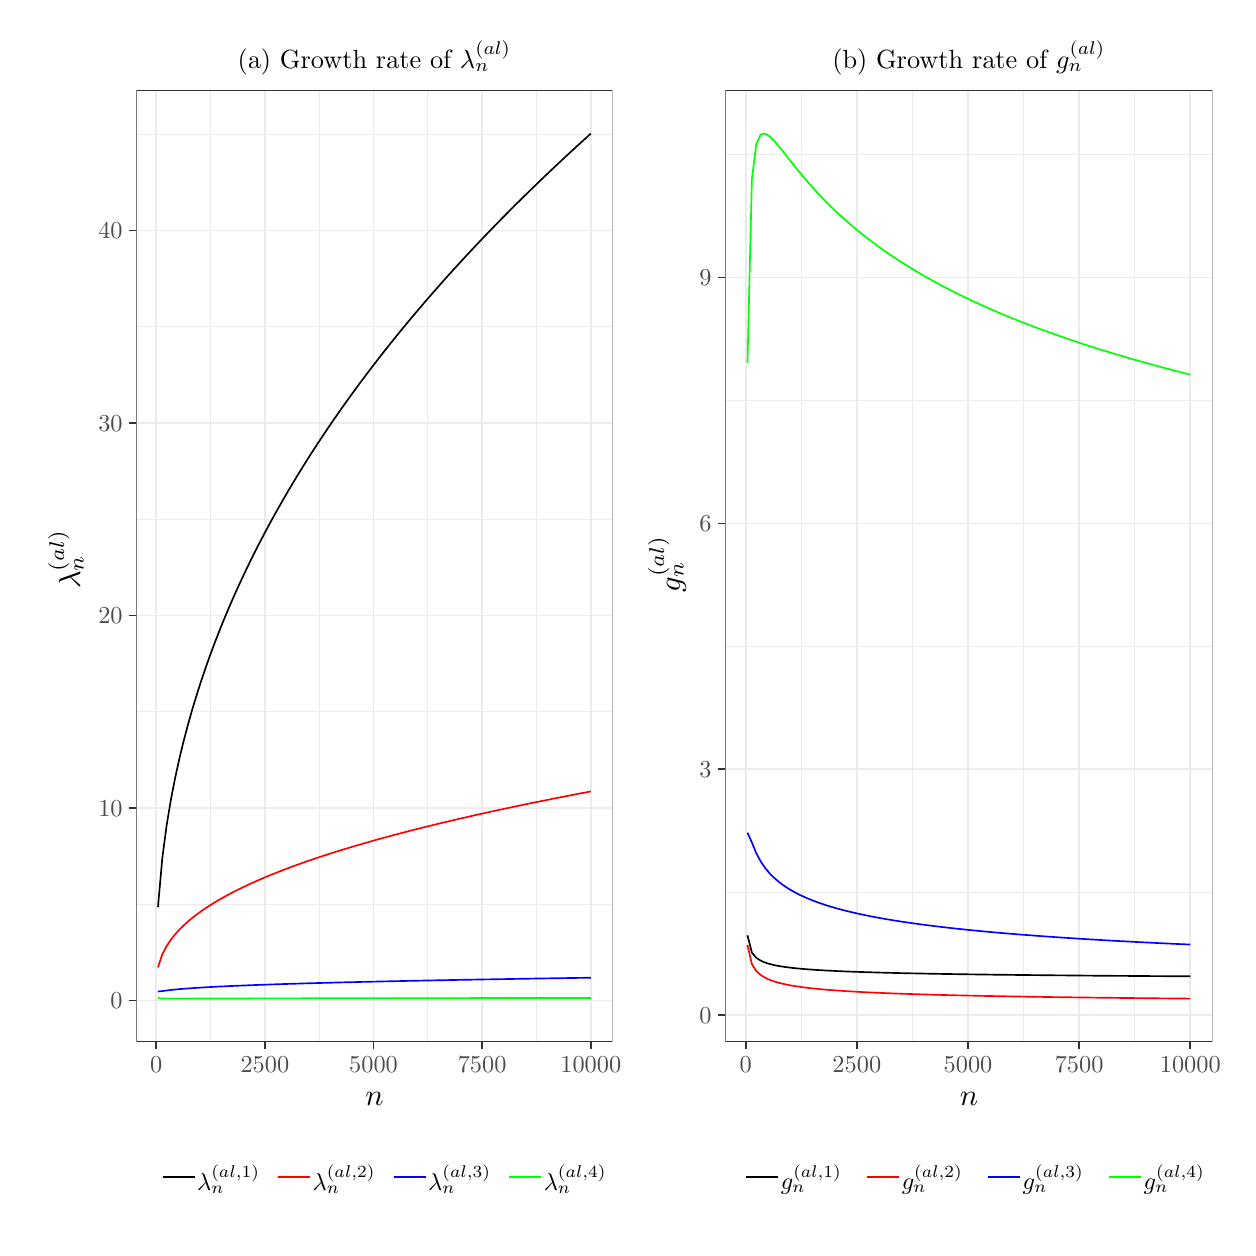
\begin{tikzpicture}[x=1pt,y=1pt]
\definecolor{fillColor}{RGB}{255,255,255}
\path[use as bounding box,fill=fillColor,fill opacity=0.00] (0,0) rectangle (433.62,433.62);
\begin{scope}
\path[clip] (  0.00,  0.00) rectangle (216.81,433.62);
\definecolor{drawColor}{RGB}{255,255,255}
\definecolor{fillColor}{RGB}{255,255,255}

\path[draw=drawColor,line width= 0.6pt,line join=round,line cap=round,fill=fillColor] (  0.00,  0.00) rectangle (216.81,433.62);
\end{scope}
\begin{scope}
\path[clip] ( 39.26, 67.14) rectangle (211.31,410.96);
\definecolor{fillColor}{RGB}{255,255,255}

\path[fill=fillColor] ( 39.26, 67.14) rectangle (211.31,410.96);
\definecolor{drawColor}{gray}{0.92}

\path[draw=drawColor,line width= 0.3pt,line join=round] ( 39.26,116.89) --
	(211.31,116.89);

\path[draw=drawColor,line width= 0.3pt,line join=round] ( 39.26,186.44) --
	(211.31,186.44);

\path[draw=drawColor,line width= 0.3pt,line join=round] ( 39.26,255.98) --
	(211.31,255.98);

\path[draw=drawColor,line width= 0.3pt,line join=round] ( 39.26,325.52) --
	(211.31,325.52);

\path[draw=drawColor,line width= 0.3pt,line join=round] ( 39.26,395.07) --
	(211.31,395.07);

\path[draw=drawColor,line width= 0.3pt,line join=round] ( 66.08, 67.14) --
	( 66.08,410.96);

\path[draw=drawColor,line width= 0.3pt,line join=round] (105.34, 67.14) --
	(105.34,410.96);

\path[draw=drawColor,line width= 0.3pt,line join=round] (144.60, 67.14) --
	(144.60,410.96);

\path[draw=drawColor,line width= 0.3pt,line join=round] (183.86, 67.14) --
	(183.86,410.96);

\path[draw=drawColor,line width= 0.6pt,line join=round] ( 39.26, 82.12) --
	(211.31, 82.12);

\path[draw=drawColor,line width= 0.6pt,line join=round] ( 39.26,151.66) --
	(211.31,151.66);

\path[draw=drawColor,line width= 0.6pt,line join=round] ( 39.26,221.21) --
	(211.31,221.21);

\path[draw=drawColor,line width= 0.6pt,line join=round] ( 39.26,290.75) --
	(211.31,290.75);

\path[draw=drawColor,line width= 0.6pt,line join=round] ( 39.26,360.30) --
	(211.31,360.30);

\path[draw=drawColor,line width= 0.6pt,line join=round] ( 46.45, 67.14) --
	( 46.45,410.96);

\path[draw=drawColor,line width= 0.6pt,line join=round] ( 85.71, 67.14) --
	( 85.71,410.96);

\path[draw=drawColor,line width= 0.6pt,line join=round] (124.97, 67.14) --
	(124.97,410.96);

\path[draw=drawColor,line width= 0.6pt,line join=round] (164.23, 67.14) --
	(164.23,410.96);

\path[draw=drawColor,line width= 0.6pt,line join=round] (203.49, 67.14) --
	(203.49,410.96);
\definecolor{drawColor}{RGB}{0,0,0}

\path[draw=drawColor,line width= 0.6pt,line join=round] ( 47.08,115.82) --
	( 48.65,133.57) --
	( 50.21,145.37) --
	( 51.77,154.76) --
	( 53.34,162.77) --
	( 54.90,169.85) --
	( 56.47,176.26) --
	( 58.03,182.16) --
	( 59.59,187.64) --
	( 61.16,192.78) --
	( 62.72,197.64) --
	( 64.29,202.25) --
	( 65.85,206.65) --
	( 67.41,210.86) --
	( 68.98,214.91) --
	( 70.54,218.81) --
	( 72.11,222.57) --
	( 73.67,226.22) --
	( 75.23,229.75) --
	( 76.80,233.18) --
	( 78.36,236.52) --
	( 79.93,239.77) --
	( 81.49,242.95) --
	( 83.05,246.04) --
	( 84.62,249.07) --
	( 86.18,252.03) --
	( 87.75,254.93) --
	( 89.31,257.77) --
	( 90.88,260.56) --
	( 92.44,263.29) --
	( 94.00,265.98) --
	( 95.57,268.62) --
	( 97.13,271.21) --
	( 98.70,273.76) --
	(100.26,276.27) --
	(101.82,278.74) --
	(103.39,281.18) --
	(104.95,283.58) --
	(106.52,285.94) --
	(108.08,288.28) --
	(109.64,290.58) --
	(111.21,292.85) --
	(112.77,295.09) --
	(114.34,297.31) --
	(115.90,299.49) --
	(117.46,301.65) --
	(119.03,303.79) --
	(120.59,305.90) --
	(122.16,307.99) --
	(123.72,310.05) --
	(125.29,312.09) --
	(126.85,314.12) --
	(128.41,316.12) --
	(129.98,318.09) --
	(131.54,320.05) --
	(133.11,322.00) --
	(134.67,323.92) --
	(136.23,325.82) --
	(137.80,327.71) --
	(139.36,329.58) --
	(140.93,331.43) --
	(142.49,333.27) --
	(144.05,335.09) --
	(145.62,336.89) --
	(147.18,338.68) --
	(148.75,340.46) --
	(150.31,342.22) --
	(151.87,343.97) --
	(153.44,345.70) --
	(155.00,347.42) --
	(156.57,349.12) --
	(158.13,350.82) --
	(159.70,352.50) --
	(161.26,354.17) --
	(162.82,355.82) --
	(164.39,357.47) --
	(165.95,359.10) --
	(167.52,360.72) --
	(169.08,362.34) --
	(170.64,363.93) --
	(172.21,365.52) --
	(173.77,367.10) --
	(175.34,368.67) --
	(176.90,370.23) --
	(178.46,371.78) --
	(180.03,373.32) --
	(181.59,374.85) --
	(183.16,376.36) --
	(184.72,377.88) --
	(186.28,379.38) --
	(187.85,380.87) --
	(189.41,382.35) --
	(190.98,383.83) --
	(192.54,385.29) --
	(194.11,386.75) --
	(195.67,388.20) --
	(197.23,389.64) --
	(198.80,391.08) --
	(200.36,392.50) --
	(201.93,393.92) --
	(203.49,395.33);
\definecolor{drawColor}{RGB}{255,0,0}

\path[draw=drawColor,line width= 0.6pt,line join=round] ( 47.08, 94.04) --
	( 48.65, 98.76) --
	( 50.21,101.76) --
	( 51.77,104.09) --
	( 53.34,106.06) --
	( 54.90,107.77) --
	( 56.47,109.31) --
	( 58.03,110.72) --
	( 59.59,112.01) --
	( 61.16,113.22) --
	( 62.72,114.36) --
	( 64.29,115.43) --
	( 65.85,116.45) --
	( 67.41,117.43) --
	( 68.98,118.36) --
	( 70.54,119.25) --
	( 72.11,120.11) --
	( 73.67,120.94) --
	( 75.23,121.75) --
	( 76.80,122.52) --
	( 78.36,123.28) --
	( 79.93,124.01) --
	( 81.49,124.73) --
	( 83.05,125.42) --
	( 84.62,126.10) --
	( 86.18,126.76) --
	( 87.75,127.41) --
	( 89.31,128.04) --
	( 90.88,128.66) --
	( 92.44,129.27) --
	( 94.00,129.86) --
	( 95.57,130.45) --
	( 97.13,131.02) --
	( 98.70,131.58) --
	(100.26,132.14) --
	(101.82,132.68) --
	(103.39,133.21) --
	(104.95,133.74) --
	(106.52,134.26) --
	(108.08,134.77) --
	(109.64,135.27) --
	(111.21,135.77) --
	(112.77,136.26) --
	(114.34,136.74) --
	(115.90,137.21) --
	(117.46,137.68) --
	(119.03,138.15) --
	(120.59,138.60) --
	(122.16,139.06) --
	(123.72,139.50) --
	(125.29,139.95) --
	(126.85,140.38) --
	(128.41,140.81) --
	(129.98,141.24) --
	(131.54,141.66) --
	(133.11,142.08) --
	(134.67,142.49) --
	(136.23,142.90) --
	(137.80,143.31) --
	(139.36,143.71) --
	(140.93,144.11) --
	(142.49,144.50) --
	(144.05,144.89) --
	(145.62,145.27) --
	(147.18,145.66) --
	(148.75,146.04) --
	(150.31,146.41) --
	(151.87,146.78) --
	(153.44,147.15) --
	(155.00,147.52) --
	(156.57,147.88) --
	(158.13,148.24) --
	(159.70,148.60) --
	(161.26,148.95) --
	(162.82,149.31) --
	(164.39,149.65) --
	(165.95,150.00) --
	(167.52,150.34) --
	(169.08,150.69) --
	(170.64,151.02) --
	(172.21,151.36) --
	(173.77,151.69) --
	(175.34,152.02) --
	(176.90,152.35) --
	(178.46,152.68) --
	(180.03,153.00) --
	(181.59,153.33) --
	(183.16,153.65) --
	(184.72,153.96) --
	(186.28,154.28) --
	(187.85,154.59) --
	(189.41,154.91) --
	(190.98,155.22) --
	(192.54,155.52) --
	(194.11,155.83) --
	(195.67,156.13) --
	(197.23,156.44) --
	(198.80,156.74) --
	(200.36,157.04) --
	(201.93,157.33) --
	(203.49,157.63);
\definecolor{drawColor}{RGB}{0,0,255}

\path[draw=drawColor,line width= 0.6pt,line join=round] ( 47.08, 85.35) --
	( 48.65, 85.49) --
	( 50.21, 85.71) --
	( 51.77, 85.89) --
	( 53.34, 86.06) --
	( 54.90, 86.20) --
	( 56.47, 86.33) --
	( 58.03, 86.45) --
	( 59.59, 86.56) --
	( 61.16, 86.67) --
	( 62.72, 86.76) --
	( 64.29, 86.86) --
	( 65.85, 86.94) --
	( 67.41, 87.03) --
	( 68.98, 87.11) --
	( 70.54, 87.18) --
	( 72.11, 87.26) --
	( 73.67, 87.33) --
	( 75.23, 87.40) --
	( 76.80, 87.46) --
	( 78.36, 87.52) --
	( 79.93, 87.59) --
	( 81.49, 87.65) --
	( 83.05, 87.71) --
	( 84.62, 87.76) --
	( 86.18, 87.82) --
	( 87.75, 87.87) --
	( 89.31, 87.93) --
	( 90.88, 87.98) --
	( 92.44, 88.03) --
	( 94.00, 88.08) --
	( 95.57, 88.13) --
	( 97.13, 88.17) --
	( 98.70, 88.22) --
	(100.26, 88.27) --
	(101.82, 88.31) --
	(103.39, 88.36) --
	(104.95, 88.40) --
	(106.52, 88.44) --
	(108.08, 88.48) --
	(109.64, 88.52) --
	(111.21, 88.57) --
	(112.77, 88.61) --
	(114.34, 88.65) --
	(115.90, 88.68) --
	(117.46, 88.72) --
	(119.03, 88.76) --
	(120.59, 88.80) --
	(122.16, 88.83) --
	(123.72, 88.87) --
	(125.29, 88.91) --
	(126.85, 88.94) --
	(128.41, 88.98) --
	(129.98, 89.01) --
	(131.54, 89.05) --
	(133.11, 89.08) --
	(134.67, 89.11) --
	(136.23, 89.15) --
	(137.80, 89.18) --
	(139.36, 89.21) --
	(140.93, 89.24) --
	(142.49, 89.28) --
	(144.05, 89.31) --
	(145.62, 89.34) --
	(147.18, 89.37) --
	(148.75, 89.40) --
	(150.31, 89.43) --
	(151.87, 89.46) --
	(153.44, 89.49) --
	(155.00, 89.52) --
	(156.57, 89.55) --
	(158.13, 89.58) --
	(159.70, 89.60) --
	(161.26, 89.63) --
	(162.82, 89.66) --
	(164.39, 89.69) --
	(165.95, 89.72) --
	(167.52, 89.74) --
	(169.08, 89.77) --
	(170.64, 89.80) --
	(172.21, 89.82) --
	(173.77, 89.85) --
	(175.34, 89.88) --
	(176.90, 89.90) --
	(178.46, 89.93) --
	(180.03, 89.95) --
	(181.59, 89.98) --
	(183.16, 90.01) --
	(184.72, 90.03) --
	(186.28, 90.06) --
	(187.85, 90.08) --
	(189.41, 90.11) --
	(190.98, 90.13) --
	(192.54, 90.15) --
	(194.11, 90.18) --
	(195.67, 90.20) --
	(197.23, 90.23) --
	(198.80, 90.25) --
	(200.36, 90.27) --
	(201.93, 90.30) --
	(203.49, 90.32);
\definecolor{drawColor}{RGB}{0,255,0}

\path[draw=drawColor,line width= 0.6pt,line join=round] ( 47.08, 83.00) --
	( 48.65, 82.80) --
	( 50.21, 82.78) --
	( 51.77, 82.77) --
	( 53.34, 82.77) --
	( 54.90, 82.77) --
	( 56.47, 82.77) --
	( 58.03, 82.78) --
	( 59.59, 82.78) --
	( 61.16, 82.79) --
	( 62.72, 82.79) --
	( 64.29, 82.79) --
	( 65.85, 82.80) --
	( 67.41, 82.80) --
	( 68.98, 82.81) --
	( 70.54, 82.81) --
	( 72.11, 82.82) --
	( 73.67, 82.82) --
	( 75.23, 82.82) --
	( 76.80, 82.83) --
	( 78.36, 82.83) --
	( 79.93, 82.83) --
	( 81.49, 82.84) --
	( 83.05, 82.84) --
	( 84.62, 82.84) --
	( 86.18, 82.85) --
	( 87.75, 82.85) --
	( 89.31, 82.85) --
	( 90.88, 82.86) --
	( 92.44, 82.86) --
	( 94.00, 82.86) --
	( 95.57, 82.87) --
	( 97.13, 82.87) --
	( 98.70, 82.87) --
	(100.26, 82.88) --
	(101.82, 82.88) --
	(103.39, 82.88) --
	(104.95, 82.88) --
	(106.52, 82.89) --
	(108.08, 82.89) --
	(109.64, 82.89) --
	(111.21, 82.90) --
	(112.77, 82.90) --
	(114.34, 82.90) --
	(115.90, 82.90) --
	(117.46, 82.91) --
	(119.03, 82.91) --
	(120.59, 82.91) --
	(122.16, 82.91) --
	(123.72, 82.92) --
	(125.29, 82.92) --
	(126.85, 82.92) --
	(128.41, 82.92) --
	(129.98, 82.92) --
	(131.54, 82.93) --
	(133.11, 82.93) --
	(134.67, 82.93) --
	(136.23, 82.93) --
	(137.80, 82.94) --
	(139.36, 82.94) --
	(140.93, 82.94) --
	(142.49, 82.94) --
	(144.05, 82.94) --
	(145.62, 82.95) --
	(147.18, 82.95) --
	(148.75, 82.95) --
	(150.31, 82.95) --
	(151.87, 82.95) --
	(153.44, 82.96) --
	(155.00, 82.96) --
	(156.57, 82.96) --
	(158.13, 82.96) --
	(159.70, 82.96) --
	(161.26, 82.97) --
	(162.82, 82.97) --
	(164.39, 82.97) --
	(165.95, 82.97) --
	(167.52, 82.97) --
	(169.08, 82.97) --
	(170.64, 82.98) --
	(172.21, 82.98) --
	(173.77, 82.98) --
	(175.34, 82.98) --
	(176.90, 82.98) --
	(178.46, 82.99) --
	(180.03, 82.99) --
	(181.59, 82.99) --
	(183.16, 82.99) --
	(184.72, 82.99) --
	(186.28, 82.99) --
	(187.85, 83.00) --
	(189.41, 83.00) --
	(190.98, 83.00) --
	(192.54, 83.00) --
	(194.11, 83.00) --
	(195.67, 83.00) --
	(197.23, 83.01) --
	(198.80, 83.01) --
	(200.36, 83.01) --
	(201.93, 83.01) --
	(203.49, 83.01);
\definecolor{drawColor}{gray}{0.20}

\path[draw=drawColor,line width= 0.6pt,line join=round,line cap=round] ( 39.26, 67.14) rectangle (211.31,410.96);
\end{scope}
\begin{scope}
\path[clip] (  0.00,  0.00) rectangle (433.62,433.62);
\definecolor{drawColor}{gray}{0.30}

\node[text=drawColor,anchor=base east,inner sep=0pt, outer sep=0pt, scale=  0.88] at ( 34.31, 79.09) {0};

\node[text=drawColor,anchor=base east,inner sep=0pt, outer sep=0pt, scale=  0.88] at ( 34.31,148.63) {10};

\node[text=drawColor,anchor=base east,inner sep=0pt, outer sep=0pt, scale=  0.88] at ( 34.31,218.18) {20};

\node[text=drawColor,anchor=base east,inner sep=0pt, outer sep=0pt, scale=  0.88] at ( 34.31,287.72) {30};

\node[text=drawColor,anchor=base east,inner sep=0pt, outer sep=0pt, scale=  0.88] at ( 34.31,357.27) {40};
\end{scope}
\begin{scope}
\path[clip] (  0.00,  0.00) rectangle (433.62,433.62);
\definecolor{drawColor}{gray}{0.20}

\path[draw=drawColor,line width= 0.6pt,line join=round] ( 36.51, 82.12) --
	( 39.26, 82.12);

\path[draw=drawColor,line width= 0.6pt,line join=round] ( 36.51,151.66) --
	( 39.26,151.66);

\path[draw=drawColor,line width= 0.6pt,line join=round] ( 36.51,221.21) --
	( 39.26,221.21);

\path[draw=drawColor,line width= 0.6pt,line join=round] ( 36.51,290.75) --
	( 39.26,290.75);

\path[draw=drawColor,line width= 0.6pt,line join=round] ( 36.51,360.30) --
	( 39.26,360.30);
\end{scope}
\begin{scope}
\path[clip] (  0.00,  0.00) rectangle (433.62,433.62);
\definecolor{drawColor}{gray}{0.20}

\path[draw=drawColor,line width= 0.6pt,line join=round] ( 46.45, 64.39) --
	( 46.45, 67.14);

\path[draw=drawColor,line width= 0.6pt,line join=round] ( 85.71, 64.39) --
	( 85.71, 67.14);

\path[draw=drawColor,line width= 0.6pt,line join=round] (124.97, 64.39) --
	(124.97, 67.14);

\path[draw=drawColor,line width= 0.6pt,line join=round] (164.23, 64.39) --
	(164.23, 67.14);

\path[draw=drawColor,line width= 0.6pt,line join=round] (203.49, 64.39) --
	(203.49, 67.14);
\end{scope}
\begin{scope}
\path[clip] (  0.00,  0.00) rectangle (433.62,433.62);
\definecolor{drawColor}{gray}{0.30}

\node[text=drawColor,anchor=base,inner sep=0pt, outer sep=0pt, scale=  0.88] at ( 46.45, 56.13) {0};

\node[text=drawColor,anchor=base,inner sep=0pt, outer sep=0pt, scale=  0.88] at ( 85.71, 56.13) {2500};

\node[text=drawColor,anchor=base,inner sep=0pt, outer sep=0pt, scale=  0.88] at (124.97, 56.13) {5000};

\node[text=drawColor,anchor=base,inner sep=0pt, outer sep=0pt, scale=  0.88] at (164.23, 56.13) {7500};

\node[text=drawColor,anchor=base,inner sep=0pt, outer sep=0pt, scale=  0.88] at (203.49, 56.13) {10000};
\end{scope}
\begin{scope}
\path[clip] (  0.00,  0.00) rectangle (433.62,433.62);
\definecolor{drawColor}{RGB}{0,0,0}

\node[text=drawColor,anchor=base,inner sep=0pt, outer sep=0pt, scale=  1.10] at (125.29, 44.09) {$n$};
\end{scope}
\begin{scope}
\path[clip] (  0.00,  0.00) rectangle (433.62,433.62);
\definecolor{drawColor}{RGB}{0,0,0}

\node[text=drawColor,rotate= 90.00,anchor=base west,inner sep=0pt, outer sep=0pt, scale=  1.10] at ( 18.91,230.79) {$\lambda_n^{(al)}$};

\end{scope}
\begin{scope}
\path[clip] (  0.00,  0.00) rectangle (433.62,433.62);
\definecolor{fillColor}{RGB}{255,255,255}

\path[fill=fillColor] ( 36.28,  5.50) rectangle (214.29, 30.95);
\end{scope}
\begin{scope}
\path[clip] (  0.00,  0.00) rectangle (433.62,433.62);
\definecolor{fillColor}{RGB}{255,255,255}

\path[fill=fillColor] ( 47.28, 11.00) rectangle ( 61.73, 25.45);
\end{scope}
\begin{scope}
\path[clip] (  0.00,  0.00) rectangle (433.62,433.62);
\definecolor{drawColor}{RGB}{0,0,0}

\path[draw=drawColor,line width= 0.6pt,line join=round] ( 48.72, 18.23) -- ( 60.29, 18.23);
\end{scope}
\begin{scope}
\path[clip] (  0.00,  0.00) rectangle (433.62,433.62);
\definecolor{drawColor}{RGB}{0,0,0}

\path[draw=drawColor,line width= 0.6pt,line join=round] ( 48.72, 18.23) -- ( 60.29, 18.23);
\end{scope}
\begin{scope}
\path[clip] (  0.00,  0.00) rectangle (433.62,433.62);
\definecolor{drawColor}{RGB}{0,0,0}

\path[draw=drawColor,line width= 0.6pt,line join=round] ( 48.72, 18.23) -- ( 60.29, 18.23);
\end{scope}
\begin{scope}
\path[clip] (  0.00,  0.00) rectangle (433.62,433.62);
\definecolor{drawColor}{RGB}{0,0,0}

\path[draw=drawColor,line width= 0.6pt,line join=round] ( 48.72, 18.23) -- ( 60.29, 18.23);
\end{scope}
\begin{scope}
\path[clip] (  0.00,  0.00) rectangle (433.62,433.62);
\definecolor{fillColor}{RGB}{255,255,255}

\path[fill=fillColor] ( 89.03, 11.00) rectangle (103.48, 25.45);
\end{scope}
\begin{scope}
\path[clip] (  0.00,  0.00) rectangle (433.62,433.62);
\definecolor{drawColor}{RGB}{255,0,0}

\path[draw=drawColor,line width= 0.6pt,line join=round] ( 90.48, 18.23) -- (102.04, 18.23);
\end{scope}
\begin{scope}
\path[clip] (  0.00,  0.00) rectangle (433.62,433.62);
\definecolor{drawColor}{RGB}{255,0,0}

\path[draw=drawColor,line width= 0.6pt,line join=round] ( 90.48, 18.23) -- (102.04, 18.23);
\end{scope}
\begin{scope}
\path[clip] (  0.00,  0.00) rectangle (433.62,433.62);
\definecolor{drawColor}{RGB}{255,0,0}

\path[draw=drawColor,line width= 0.6pt,line join=round] ( 90.48, 18.23) -- (102.04, 18.23);
\end{scope}
\begin{scope}
\path[clip] (  0.00,  0.00) rectangle (433.62,433.62);
\definecolor{drawColor}{RGB}{255,0,0}

\path[draw=drawColor,line width= 0.6pt,line join=round] ( 90.48, 18.23) -- (102.04, 18.23);
\end{scope}
\begin{scope}
\path[clip] (  0.00,  0.00) rectangle (433.62,433.62);
\definecolor{fillColor}{RGB}{255,255,255}

\path[fill=fillColor] (130.79, 11.00) rectangle (145.24, 25.45);
\end{scope}
\begin{scope}
\path[clip] (  0.00,  0.00) rectangle (433.62,433.62);
\definecolor{drawColor}{RGB}{0,0,255}

\path[draw=drawColor,line width= 0.6pt,line join=round] (132.23, 18.23) -- (143.79, 18.23);
\end{scope}
\begin{scope}
\path[clip] (  0.00,  0.00) rectangle (433.62,433.62);
\definecolor{drawColor}{RGB}{0,0,255}

\path[draw=drawColor,line width= 0.6pt,line join=round] (132.23, 18.23) -- (143.79, 18.23);
\end{scope}
\begin{scope}
\path[clip] (  0.00,  0.00) rectangle (433.62,433.62);
\definecolor{drawColor}{RGB}{0,0,255}

\path[draw=drawColor,line width= 0.6pt,line join=round] (132.23, 18.23) -- (143.79, 18.23);
\end{scope}
\begin{scope}
\path[clip] (  0.00,  0.00) rectangle (433.62,433.62);
\definecolor{drawColor}{RGB}{0,0,255}

\path[draw=drawColor,line width= 0.6pt,line join=round] (132.23, 18.23) -- (143.79, 18.23);
\end{scope}
\begin{scope}
\path[clip] (  0.00,  0.00) rectangle (433.62,433.62);
\definecolor{fillColor}{RGB}{255,255,255}

\path[fill=fillColor] (172.54, 11.00) rectangle (186.99, 25.45);
\end{scope}
\begin{scope}
\path[clip] (  0.00,  0.00) rectangle (433.62,433.62);
\definecolor{drawColor}{RGB}{0,255,0}

\path[draw=drawColor,line width= 0.6pt,line join=round] (173.99, 18.23) -- (185.55, 18.23);
\end{scope}
\begin{scope}
\path[clip] (  0.00,  0.00) rectangle (433.62,433.62);
\definecolor{drawColor}{RGB}{0,255,0}

\path[draw=drawColor,line width= 0.6pt,line join=round] (173.99, 18.23) -- (185.55, 18.23);
\end{scope}
\begin{scope}
\path[clip] (  0.00,  0.00) rectangle (433.62,433.62);
\definecolor{drawColor}{RGB}{0,255,0}

\path[draw=drawColor,line width= 0.6pt,line join=round] (173.99, 18.23) -- (185.55, 18.23);
\end{scope}
\begin{scope}
\path[clip] (  0.00,  0.00) rectangle (433.62,433.62);
\definecolor{drawColor}{RGB}{0,255,0}

\path[draw=drawColor,line width= 0.6pt,line join=round] (173.99, 18.23) -- (185.55, 18.23);
\end{scope}
\begin{scope}
\path[clip] (  0.00,  0.00) rectangle (433.62,433.62);
\definecolor{drawColor}{RGB}{0,0,0}

\node[text=drawColor,anchor=base west,inner sep=0pt, outer sep=0pt, scale=  0.88] at ( 61.23, 13.55) {$\lambda_n^{(al, 1)}$};

\end{scope}
\begin{scope}
\path[clip] (  0.00,  0.00) rectangle (433.62,433.62);
\definecolor{drawColor}{RGB}{0,0,0}

\node[text=drawColor,anchor=base west,inner sep=0pt, outer sep=0pt, scale=  0.88] at (102.98, 13.55) {$\lambda_n^{(al, 2)}$};

\end{scope}
\begin{scope}
\path[clip] (  0.00,  0.00) rectangle (433.62,433.62);
\definecolor{drawColor}{RGB}{0,0,0}

\node[text=drawColor,anchor=base west,inner sep=0pt, outer sep=0pt, scale=  0.88] at (144.74, 13.55) {$\lambda_n^{(al, 3)}$};

\end{scope}
\begin{scope}
\path[clip] (  0.00,  0.00) rectangle (433.62,433.62);
\definecolor{drawColor}{RGB}{0,0,0}

\node[text=drawColor,anchor=base west,inner sep=0pt, outer sep=0pt, scale=  0.88] at (186.49, 13.55) {$\lambda_n^{(al, 4)}$};

\end{scope}
\begin{scope}
\path[clip] (  0.00,  0.00) rectangle (433.62,433.62);
\definecolor{drawColor}{RGB}{0,0,0}

\node[text=drawColor,anchor=base,inner sep=0pt, outer sep=0pt, scale=  0.95] at (125.29,419.03) {(a) Growth rate of $\lambda_n^{(al)}$};
\end{scope}
\begin{scope}
\path[clip] (216.81,  0.00) rectangle (433.62,433.62);
\definecolor{drawColor}{RGB}{255,255,255}
\definecolor{fillColor}{RGB}{255,255,255}

\path[draw=drawColor,line width= 0.6pt,line join=round,line cap=round,fill=fillColor] (216.81,  0.00) rectangle (433.62,433.62);
\end{scope}
\begin{scope}
\path[clip] (252.10, 67.14) rectangle (428.12,410.96);
\definecolor{fillColor}{RGB}{255,255,255}

\path[fill=fillColor] (252.10, 67.14) rectangle (428.12,410.96);
\definecolor{drawColor}{gray}{0.92}

\path[draw=drawColor,line width= 0.3pt,line join=round] (252.10,121.25) --
	(428.12,121.25);

\path[draw=drawColor,line width= 0.3pt,line join=round] (252.10,210.09) --
	(428.12,210.09);

\path[draw=drawColor,line width= 0.3pt,line join=round] (252.10,298.93) --
	(428.12,298.93);

\path[draw=drawColor,line width= 0.3pt,line join=round] (252.10,387.77) --
	(428.12,387.77);

\path[draw=drawColor,line width= 0.3pt,line join=round] (279.54, 67.14) --
	(279.54,410.96);

\path[draw=drawColor,line width= 0.3pt,line join=round] (319.70, 67.14) --
	(319.70,410.96);

\path[draw=drawColor,line width= 0.3pt,line join=round] (359.87, 67.14) --
	(359.87,410.96);

\path[draw=drawColor,line width= 0.3pt,line join=round] (400.04, 67.14) --
	(400.04,410.96);

\path[draw=drawColor,line width= 0.6pt,line join=round] (252.10, 76.83) --
	(428.12, 76.83);

\path[draw=drawColor,line width= 0.6pt,line join=round] (252.10,165.67) --
	(428.12,165.67);

\path[draw=drawColor,line width= 0.6pt,line join=round] (252.10,254.51) --
	(428.12,254.51);

\path[draw=drawColor,line width= 0.6pt,line join=round] (252.10,343.35) --
	(428.12,343.35);

\path[draw=drawColor,line width= 0.6pt,line join=round] (259.45, 67.14) --
	(259.45,410.96);

\path[draw=drawColor,line width= 0.6pt,line join=round] (299.62, 67.14) --
	(299.62,410.96);

\path[draw=drawColor,line width= 0.6pt,line join=round] (339.79, 67.14) --
	(339.79,410.96);

\path[draw=drawColor,line width= 0.6pt,line join=round] (379.95, 67.14) --
	(379.95,410.96);

\path[draw=drawColor,line width= 0.6pt,line join=round] (420.12, 67.14) --
	(420.12,410.96);
\definecolor{drawColor}{RGB}{0,0,0}

\path[draw=drawColor,line width= 0.6pt,line join=round] (260.10,105.62) --
	(261.70, 99.37) --
	(263.30, 97.50) --
	(264.90, 96.47) --
	(266.50, 95.78) --
	(268.10, 95.28) --
	(269.70, 94.89) --
	(271.30, 94.57) --
	(272.90, 94.31) --
	(274.50, 94.09) --
	(276.10, 93.89) --
	(277.70, 93.72) --
	(279.30, 93.57) --
	(280.90, 93.43) --
	(282.50, 93.31) --
	(284.10, 93.19) --
	(285.70, 93.09) --
	(287.30, 92.99) --
	(288.90, 92.90) --
	(290.50, 92.82) --
	(292.10, 92.74) --
	(293.70, 92.67) --
	(295.30, 92.60) --
	(296.90, 92.54) --
	(298.50, 92.48) --
	(300.10, 92.42) --
	(301.70, 92.37) --
	(303.30, 92.32) --
	(304.90, 92.27) --
	(306.50, 92.22) --
	(308.10, 92.17) --
	(309.70, 92.13) --
	(311.30, 92.09) --
	(312.90, 92.05) --
	(314.50, 92.01) --
	(316.10, 91.97) --
	(317.71, 91.94) --
	(319.31, 91.90) --
	(320.91, 91.87) --
	(322.51, 91.84) --
	(324.11, 91.81) --
	(325.71, 91.78) --
	(327.31, 91.75) --
	(328.91, 91.72) --
	(330.51, 91.69) --
	(332.11, 91.67) --
	(333.71, 91.64) --
	(335.31, 91.61) --
	(336.91, 91.59) --
	(338.51, 91.57) --
	(340.11, 91.54) --
	(341.71, 91.52) --
	(343.31, 91.50) --
	(344.91, 91.48) --
	(346.51, 91.46) --
	(348.11, 91.43) --
	(349.71, 91.41) --
	(351.31, 91.40) --
	(352.91, 91.38) --
	(354.51, 91.36) --
	(356.11, 91.34) --
	(357.71, 91.32) --
	(359.31, 91.30) --
	(360.91, 91.29) --
	(362.51, 91.27) --
	(364.11, 91.25) --
	(365.71, 91.24) --
	(367.31, 91.22) --
	(368.91, 91.20) --
	(370.51, 91.19) --
	(372.11, 91.17) --
	(373.71, 91.16) --
	(375.31, 91.15) --
	(376.91, 91.13) --
	(378.51, 91.12) --
	(380.11, 91.10) --
	(381.71, 91.09) --
	(383.31, 91.08) --
	(384.91, 91.06) --
	(386.51, 91.05) --
	(388.11, 91.04) --
	(389.71, 91.03) --
	(391.32, 91.01) --
	(392.92, 91.00) --
	(394.52, 90.99) --
	(396.12, 90.98) --
	(397.72, 90.97) --
	(399.32, 90.95) --
	(400.92, 90.94) --
	(402.52, 90.93) --
	(404.12, 90.92) --
	(405.72, 90.91) --
	(407.32, 90.90) --
	(408.92, 90.89) --
	(410.52, 90.88) --
	(412.12, 90.87) --
	(413.72, 90.86) --
	(415.32, 90.85) --
	(416.92, 90.84) --
	(418.52, 90.83) --
	(420.12, 90.82);
\definecolor{drawColor}{RGB}{255,0,0}

\path[draw=drawColor,line width= 0.6pt,line join=round] (260.10,102.13) --
	(261.70, 95.20) --
	(263.30, 92.72) --
	(264.90, 91.28) --
	(266.50, 90.30) --
	(268.10, 89.56) --
	(269.70, 88.98) --
	(271.30, 88.51) --
	(272.90, 88.12) --
	(274.50, 87.77) --
	(276.10, 87.48) --
	(277.70, 87.22) --
	(279.30, 86.98) --
	(280.90, 86.77) --
	(282.50, 86.58) --
	(284.10, 86.41) --
	(285.70, 86.25) --
	(287.30, 86.10) --
	(288.90, 85.96) --
	(290.50, 85.84) --
	(292.10, 85.72) --
	(293.70, 85.61) --
	(295.30, 85.50) --
	(296.90, 85.40) --
	(298.50, 85.31) --
	(300.10, 85.22) --
	(301.70, 85.13) --
	(303.30, 85.05) --
	(304.90, 84.98) --
	(306.50, 84.90) --
	(308.10, 84.83) --
	(309.70, 84.77) --
	(311.30, 84.70) --
	(312.90, 84.64) --
	(314.50, 84.58) --
	(316.10, 84.52) --
	(317.71, 84.47) --
	(319.31, 84.42) --
	(320.91, 84.37) --
	(322.51, 84.32) --
	(324.11, 84.27) --
	(325.71, 84.22) --
	(327.31, 84.18) --
	(328.91, 84.13) --
	(330.51, 84.09) --
	(332.11, 84.05) --
	(333.71, 84.01) --
	(335.31, 83.97) --
	(336.91, 83.93) --
	(338.51, 83.90) --
	(340.11, 83.86) --
	(341.71, 83.83) --
	(343.31, 83.79) --
	(344.91, 83.76) --
	(346.51, 83.73) --
	(348.11, 83.70) --
	(349.71, 83.67) --
	(351.31, 83.64) --
	(352.91, 83.61) --
	(354.51, 83.58) --
	(356.11, 83.55) --
	(357.71, 83.52) --
	(359.31, 83.50) --
	(360.91, 83.47) --
	(362.51, 83.44) --
	(364.11, 83.42) --
	(365.71, 83.40) --
	(367.31, 83.37) --
	(368.91, 83.35) --
	(370.51, 83.32) --
	(372.11, 83.30) --
	(373.71, 83.28) --
	(375.31, 83.26) --
	(376.91, 83.24) --
	(378.51, 83.21) --
	(380.11, 83.19) --
	(381.71, 83.17) --
	(383.31, 83.15) --
	(384.91, 83.13) --
	(386.51, 83.11) --
	(388.11, 83.09) --
	(389.71, 83.08) --
	(391.32, 83.06) --
	(392.92, 83.04) --
	(394.52, 83.02) --
	(396.12, 83.00) --
	(397.72, 82.99) --
	(399.32, 82.97) --
	(400.92, 82.95) --
	(402.52, 82.94) --
	(404.12, 82.92) --
	(405.72, 82.90) --
	(407.32, 82.89) --
	(408.92, 82.87) --
	(410.52, 82.86) --
	(412.12, 82.84) --
	(413.72, 82.83) --
	(415.32, 82.81) --
	(416.92, 82.80) --
	(418.52, 82.78) --
	(420.12, 82.77);
\definecolor{drawColor}{RGB}{0,0,255}

\path[draw=drawColor,line width= 0.6pt,line join=round] (260.10,142.72) --
	(261.70,139.17) --
	(263.30,135.26) --
	(264.90,132.30) --
	(266.50,129.96) --
	(268.10,128.05) --
	(269.70,126.44) --
	(271.30,125.06) --
	(272.90,123.84) --
	(274.50,122.76) --
	(276.10,121.79) --
	(277.70,120.91) --
	(279.30,120.11) --
	(280.90,119.38) --
	(282.50,118.70) --
	(284.10,118.06) --
	(285.70,117.47) --
	(287.30,116.92) --
	(288.90,116.40) --
	(290.50,115.91) --
	(292.10,115.45) --
	(293.70,115.01) --
	(295.30,114.59) --
	(296.90,114.20) --
	(298.50,113.82) --
	(300.10,113.46) --
	(301.70,113.11) --
	(303.30,112.78) --
	(304.90,112.46) --
	(306.50,112.16) --
	(308.10,111.86) --
	(309.70,111.58) --
	(311.30,111.31) --
	(312.90,111.04) --
	(314.50,110.79) --
	(316.10,110.54) --
	(317.71,110.30) --
	(319.31,110.07) --
	(320.91,109.85) --
	(322.51,109.63) --
	(324.11,109.42) --
	(325.71,109.21) --
	(327.31,109.01) --
	(328.91,108.82) --
	(330.51,108.63) --
	(332.11,108.44) --
	(333.71,108.26) --
	(335.31,108.08) --
	(336.91,107.91) --
	(338.51,107.75) --
	(340.11,107.58) --
	(341.71,107.42) --
	(343.31,107.27) --
	(344.91,107.11) --
	(346.51,106.96) --
	(348.11,106.82) --
	(349.71,106.67) --
	(351.31,106.53) --
	(352.91,106.40) --
	(354.51,106.26) --
	(356.11,106.13) --
	(357.71,106.00) --
	(359.31,105.87) --
	(360.91,105.75) --
	(362.51,105.63) --
	(364.11,105.51) --
	(365.71,105.39) --
	(367.31,105.27) --
	(368.91,105.16) --
	(370.51,105.05) --
	(372.11,104.94) --
	(373.71,104.83) --
	(375.31,104.72) --
	(376.91,104.62) --
	(378.51,104.51) --
	(380.11,104.41) --
	(381.71,104.31) --
	(383.31,104.21) --
	(384.91,104.12) --
	(386.51,104.02) --
	(388.11,103.93) --
	(389.71,103.83) --
	(391.32,103.74) --
	(392.92,103.65) --
	(394.52,103.56) --
	(396.12,103.48) --
	(397.72,103.39) --
	(399.32,103.31) --
	(400.92,103.22) --
	(402.52,103.14) --
	(404.12,103.06) --
	(405.72,102.98) --
	(407.32,102.90) --
	(408.92,102.82) --
	(410.52,102.74) --
	(412.12,102.66) --
	(413.72,102.59) --
	(415.32,102.51) --
	(416.92,102.44) --
	(418.52,102.37) --
	(420.12,102.30);
\definecolor{drawColor}{RGB}{0,255,0}

\path[draw=drawColor,line width= 0.6pt,line join=round] (260.10,312.46) --
	(261.70,379.01) --
	(263.30,391.65) --
	(264.90,395.03) --
	(266.50,395.33) --
	(268.10,394.35) --
	(269.70,392.77) --
	(271.30,390.91) --
	(272.90,388.92) --
	(274.50,386.89) --
	(276.10,384.86) --
	(277.70,382.87) --
	(279.30,380.91) --
	(280.90,379.01) --
	(282.50,377.16) --
	(284.10,375.37) --
	(285.70,373.63) --
	(287.30,371.94) --
	(288.90,370.31) --
	(290.50,368.73) --
	(292.10,367.19) --
	(293.70,365.70) --
	(295.30,364.26) --
	(296.90,362.86) --
	(298.50,361.49) --
	(300.10,360.17) --
	(301.70,358.88) --
	(303.30,357.62) --
	(304.90,356.40) --
	(306.50,355.21) --
	(308.10,354.05) --
	(309.70,352.91) --
	(311.30,351.81) --
	(312.90,350.73) --
	(314.50,349.67) --
	(316.10,348.64) --
	(317.71,347.63) --
	(319.31,346.65) --
	(320.91,345.68) --
	(322.51,344.74) --
	(324.11,343.81) --
	(325.71,342.91) --
	(327.31,342.02) --
	(328.91,341.15) --
	(330.51,340.29) --
	(332.11,339.45) --
	(333.71,338.63) --
	(335.31,337.82) --
	(336.91,337.03) --
	(338.51,336.25) --
	(340.11,335.48) --
	(341.71,334.73) --
	(343.31,333.99) --
	(344.91,333.26) --
	(346.51,332.55) --
	(348.11,331.84) --
	(349.71,331.15) --
	(351.31,330.46) --
	(352.91,329.79) --
	(354.51,329.13) --
	(356.11,328.48) --
	(357.71,327.84) --
	(359.31,327.20) --
	(360.91,326.58) --
	(362.51,325.97) --
	(364.11,325.36) --
	(365.71,324.76) --
	(367.31,324.17) --
	(368.91,323.59) --
	(370.51,323.02) --
	(372.11,322.45) --
	(373.71,321.89) --
	(375.31,321.34) --
	(376.91,320.79) --
	(378.51,320.26) --
	(380.11,319.73) --
	(381.71,319.20) --
	(383.31,318.68) --
	(384.91,318.17) --
	(386.51,317.66) --
	(388.11,317.16) --
	(389.71,316.67) --
	(391.32,316.18) --
	(392.92,315.70) --
	(394.52,315.22) --
	(396.12,314.75) --
	(397.72,314.28) --
	(399.32,313.82) --
	(400.92,313.37) --
	(402.52,312.91) --
	(404.12,312.47) --
	(405.72,312.02) --
	(407.32,311.59) --
	(408.92,311.15) --
	(410.52,310.72) --
	(412.12,310.30) --
	(413.72,309.88) --
	(415.32,309.46) --
	(416.92,309.05) --
	(418.52,308.65) --
	(420.12,308.24);
\definecolor{drawColor}{gray}{0.20}

\path[draw=drawColor,line width= 0.6pt,line join=round,line cap=round] (252.10, 67.14) rectangle (428.12,410.96);
\end{scope}
\begin{scope}
\path[clip] (  0.00,  0.00) rectangle (433.62,433.62);
\definecolor{drawColor}{gray}{0.30}

\node[text=drawColor,anchor=base east,inner sep=0pt, outer sep=0pt, scale=  0.88] at (247.15, 73.79) {0};

\node[text=drawColor,anchor=base east,inner sep=0pt, outer sep=0pt, scale=  0.88] at (247.15,162.64) {3};

\node[text=drawColor,anchor=base east,inner sep=0pt, outer sep=0pt, scale=  0.88] at (247.15,251.48) {6};

\node[text=drawColor,anchor=base east,inner sep=0pt, outer sep=0pt, scale=  0.88] at (247.15,340.32) {9};
\end{scope}
\begin{scope}
\path[clip] (  0.00,  0.00) rectangle (433.62,433.62);
\definecolor{drawColor}{gray}{0.20}

\path[draw=drawColor,line width= 0.6pt,line join=round] (249.35, 76.83) --
	(252.10, 76.83);

\path[draw=drawColor,line width= 0.6pt,line join=round] (249.35,165.67) --
	(252.10,165.67);

\path[draw=drawColor,line width= 0.6pt,line join=round] (249.35,254.51) --
	(252.10,254.51);

\path[draw=drawColor,line width= 0.6pt,line join=round] (249.35,343.35) --
	(252.10,343.35);
\end{scope}
\begin{scope}
\path[clip] (  0.00,  0.00) rectangle (433.62,433.62);
\definecolor{drawColor}{gray}{0.20}

\path[draw=drawColor,line width= 0.6pt,line join=round] (259.45, 64.39) --
	(259.45, 67.14);

\path[draw=drawColor,line width= 0.6pt,line join=round] (299.62, 64.39) --
	(299.62, 67.14);

\path[draw=drawColor,line width= 0.6pt,line join=round] (339.79, 64.39) --
	(339.79, 67.14);

\path[draw=drawColor,line width= 0.6pt,line join=round] (379.95, 64.39) --
	(379.95, 67.14);

\path[draw=drawColor,line width= 0.6pt,line join=round] (420.12, 64.39) --
	(420.12, 67.14);
\end{scope}
\begin{scope}
\path[clip] (  0.00,  0.00) rectangle (433.62,433.62);
\definecolor{drawColor}{gray}{0.30}

\node[text=drawColor,anchor=base,inner sep=0pt, outer sep=0pt, scale=  0.88] at (259.45, 56.13) {0};

\node[text=drawColor,anchor=base,inner sep=0pt, outer sep=0pt, scale=  0.88] at (299.62, 56.13) {2500};

\node[text=drawColor,anchor=base,inner sep=0pt, outer sep=0pt, scale=  0.88] at (339.79, 56.13) {5000};

\node[text=drawColor,anchor=base,inner sep=0pt, outer sep=0pt, scale=  0.88] at (379.95, 56.13) {7500};

\node[text=drawColor,anchor=base,inner sep=0pt, outer sep=0pt, scale=  0.88] at (420.12, 56.13) {10000};
\end{scope}
\begin{scope}
\path[clip] (  0.00,  0.00) rectangle (433.62,433.62);
\definecolor{drawColor}{RGB}{0,0,0}

\node[text=drawColor,anchor=base,inner sep=0pt, outer sep=0pt, scale=  1.10] at (340.11, 44.09) {$n$};
\end{scope}
\begin{scope}
\path[clip] (  0.00,  0.00) rectangle (433.62,433.62);
\definecolor{drawColor}{RGB}{0,0,0}

\node[text=drawColor,rotate= 90.00,anchor=base west,inner sep=0pt, outer sep=0pt, scale=  1.10] at (235.72,229.57) {$g_n^{(al)}$};

\end{scope}
\begin{scope}
\path[clip] (  0.00,  0.00) rectangle (433.62,433.62);
\definecolor{fillColor}{RGB}{255,255,255}

\path[fill=fillColor] (247.19,  5.50) rectangle (433.03, 30.95);
\end{scope}
\begin{scope}
\path[clip] (  0.00,  0.00) rectangle (433.62,433.62);
\definecolor{fillColor}{RGB}{255,255,255}

\path[fill=fillColor] (258.19, 11.00) rectangle (272.64, 25.45);
\end{scope}
\begin{scope}
\path[clip] (  0.00,  0.00) rectangle (433.62,433.62);
\definecolor{drawColor}{RGB}{0,0,0}

\path[draw=drawColor,line width= 0.6pt,line join=round] (259.63, 18.23) -- (271.20, 18.23);
\end{scope}
\begin{scope}
\path[clip] (  0.00,  0.00) rectangle (433.62,433.62);
\definecolor{drawColor}{RGB}{0,0,0}

\path[draw=drawColor,line width= 0.6pt,line join=round] (259.63, 18.23) -- (271.20, 18.23);
\end{scope}
\begin{scope}
\path[clip] (  0.00,  0.00) rectangle (433.62,433.62);
\definecolor{drawColor}{RGB}{0,0,0}

\path[draw=drawColor,line width= 0.6pt,line join=round] (259.63, 18.23) -- (271.20, 18.23);
\end{scope}
\begin{scope}
\path[clip] (  0.00,  0.00) rectangle (433.62,433.62);
\definecolor{drawColor}{RGB}{0,0,0}

\path[draw=drawColor,line width= 0.6pt,line join=round] (259.63, 18.23) -- (271.20, 18.23);
\end{scope}
\begin{scope}
\path[clip] (  0.00,  0.00) rectangle (433.62,433.62);
\definecolor{fillColor}{RGB}{255,255,255}

\path[fill=fillColor] (301.90, 11.00) rectangle (316.35, 25.45);
\end{scope}
\begin{scope}
\path[clip] (  0.00,  0.00) rectangle (433.62,433.62);
\definecolor{drawColor}{RGB}{255,0,0}

\path[draw=drawColor,line width= 0.6pt,line join=round] (303.34, 18.23) -- (314.91, 18.23);
\end{scope}
\begin{scope}
\path[clip] (  0.00,  0.00) rectangle (433.62,433.62);
\definecolor{drawColor}{RGB}{255,0,0}

\path[draw=drawColor,line width= 0.6pt,line join=round] (303.34, 18.23) -- (314.91, 18.23);
\end{scope}
\begin{scope}
\path[clip] (  0.00,  0.00) rectangle (433.62,433.62);
\definecolor{drawColor}{RGB}{255,0,0}

\path[draw=drawColor,line width= 0.6pt,line join=round] (303.34, 18.23) -- (314.91, 18.23);
\end{scope}
\begin{scope}
\path[clip] (  0.00,  0.00) rectangle (433.62,433.62);
\definecolor{drawColor}{RGB}{255,0,0}

\path[draw=drawColor,line width= 0.6pt,line join=round] (303.34, 18.23) -- (314.91, 18.23);
\end{scope}
\begin{scope}
\path[clip] (  0.00,  0.00) rectangle (433.62,433.62);
\definecolor{fillColor}{RGB}{255,255,255}

\path[fill=fillColor] (345.61, 11.00) rectangle (360.06, 25.45);
\end{scope}
\begin{scope}
\path[clip] (  0.00,  0.00) rectangle (433.62,433.62);
\definecolor{drawColor}{RGB}{0,0,255}

\path[draw=drawColor,line width= 0.6pt,line join=round] (347.05, 18.23) -- (358.62, 18.23);
\end{scope}
\begin{scope}
\path[clip] (  0.00,  0.00) rectangle (433.62,433.62);
\definecolor{drawColor}{RGB}{0,0,255}

\path[draw=drawColor,line width= 0.6pt,line join=round] (347.05, 18.23) -- (358.62, 18.23);
\end{scope}
\begin{scope}
\path[clip] (  0.00,  0.00) rectangle (433.62,433.62);
\definecolor{drawColor}{RGB}{0,0,255}

\path[draw=drawColor,line width= 0.6pt,line join=round] (347.05, 18.23) -- (358.62, 18.23);
\end{scope}
\begin{scope}
\path[clip] (  0.00,  0.00) rectangle (433.62,433.62);
\definecolor{drawColor}{RGB}{0,0,255}

\path[draw=drawColor,line width= 0.6pt,line join=round] (347.05, 18.23) -- (358.62, 18.23);
\end{scope}
\begin{scope}
\path[clip] (  0.00,  0.00) rectangle (433.62,433.62);
\definecolor{fillColor}{RGB}{255,255,255}

\path[fill=fillColor] (389.32, 11.00) rectangle (403.77, 25.45);
\end{scope}
\begin{scope}
\path[clip] (  0.00,  0.00) rectangle (433.62,433.62);
\definecolor{drawColor}{RGB}{0,255,0}

\path[draw=drawColor,line width= 0.6pt,line join=round] (390.76, 18.23) -- (402.33, 18.23);
\end{scope}
\begin{scope}
\path[clip] (  0.00,  0.00) rectangle (433.62,433.62);
\definecolor{drawColor}{RGB}{0,255,0}

\path[draw=drawColor,line width= 0.6pt,line join=round] (390.76, 18.23) -- (402.33, 18.23);
\end{scope}
\begin{scope}
\path[clip] (  0.00,  0.00) rectangle (433.62,433.62);
\definecolor{drawColor}{RGB}{0,255,0}

\path[draw=drawColor,line width= 0.6pt,line join=round] (390.76, 18.23) -- (402.33, 18.23);
\end{scope}
\begin{scope}
\path[clip] (  0.00,  0.00) rectangle (433.62,433.62);
\definecolor{drawColor}{RGB}{0,255,0}

\path[draw=drawColor,line width= 0.6pt,line join=round] (390.76, 18.23) -- (402.33, 18.23);
\end{scope}
\begin{scope}
\path[clip] (  0.00,  0.00) rectangle (433.62,433.62);
\definecolor{drawColor}{RGB}{0,0,0}

\node[text=drawColor,anchor=base west,inner sep=0pt, outer sep=0pt, scale=  0.88] at (272.14, 13.72) {$g_n^{(al,1)}$};

\end{scope}
\begin{scope}
\path[clip] (  0.00,  0.00) rectangle (433.62,433.62);
\definecolor{drawColor}{RGB}{0,0,0}

\node[text=drawColor,anchor=base west,inner sep=0pt, outer sep=0pt, scale=  0.88] at (315.85, 13.72) {$g_n^{(al,2)}$};

\end{scope}
\begin{scope}
\path[clip] (  0.00,  0.00) rectangle (433.62,433.62);
\definecolor{drawColor}{RGB}{0,0,0}

\node[text=drawColor,anchor=base west,inner sep=0pt, outer sep=0pt, scale=  0.88] at (359.56, 13.72) {$g_n^{(al,3)}$};

\end{scope}
\begin{scope}
\path[clip] (  0.00,  0.00) rectangle (433.62,433.62);
\definecolor{drawColor}{RGB}{0,0,0}

\node[text=drawColor,anchor=base west,inner sep=0pt, outer sep=0pt, scale=  0.88] at (403.27, 13.72) {$g_n^{(al,4)}$};

\end{scope}
\begin{scope}
\path[clip] (  0.00,  0.00) rectangle (433.62,433.62);
\definecolor{drawColor}{RGB}{0,0,0}

\node[text=drawColor,anchor=base,inner sep=0pt, outer sep=0pt, scale=  0.95] at (340.11,419.03) {(b) Growth rate of $g_n^{(al)}$};
\end{scope}
\end{tikzpicture}
}
	\end{center}
\end{figure}

As shown in Figure \ref{fig:1}, $ \lambda_n^{(al, 1)} $ is the fastest-growing sequence that satisfies \eqref{eq:9}, followed by $ \lambda_n^{(al, 2)} $, and $ \lambda_n^{(al, 3)} $, where as $ \lambda_n^{(al, 4)} $ is the slowest-growing sequence, that it in fact barely converges at all. Additionally, $ g_n^{(al, 4)} $ also takes too long to converge to zero, and only converges after $ n $ reaching around 400. We will later see the effect of different convergence rates on estimators' performance. 

\begin{table}[]\center \small
\caption{Mean Prediction Square Error}
\label{tab:1}
\small
\begin{tabular}{cccccccccc}
\hline
\multicolumn{1}{|c|}{\multirow{2}{*}{$ n $}} & \multirow{2}{*}{Oracle} & \multicolumn{1}{c|}{\multirow{2}{*}{OLS}} & \multicolumn{4}{c|}{Alasso}                                                                                                & \multicolumn{3}{c|}{Lasso}                                                                       \\
\multicolumn{1}{|c|}{}                       &                         & \multicolumn{1}{c|}{}                     & $ \lambda_n^{(al, 1)} $ & $ \lambda_n^{(al, 2)} $ & $ \lambda_n^{(al, 3)} $ & \multicolumn{1}{c|}{$ \lambda_n^{(al, 4)} $} & $ \lambda_n^{(pl, 1)} $ & $ \lambda_n^{(pl, 2)} $ & \multicolumn{1}{c|}{$ \lambda_n^{(pl, 3)} $} \\ \hline
\multicolumn{1}{|c|}{40}                     & 1.3839                  & \multicolumn{1}{c|}{1.6221}               & 1.5201                  & \textbf{1.4618}         & 1.5088                  & \multicolumn{1}{c|}{1.5651}                  & 1.7574                  & 1.6333                  & \multicolumn{1}{c|}{1.5842}                  \\
\multicolumn{1}{|c|}{80}                     & 1.1545                  & \multicolumn{1}{c|}{1.2621}               & 1.5223                  & 1.3125                  & \textbf{1.2233}         & \multicolumn{1}{c|}{1.2376}                  & 1.8643                  & 1.7277                  & \multicolumn{1}{c|}{1.6190}                  \\
\multicolumn{1}{|c|}{160}                    & 1.0391                  & \multicolumn{1}{c|}{1.0568}               & 1.4095                  & 1.1578                  & 1.0609                  & \multicolumn{1}{c|}{\textbf{1.0501}}         & 1.6813                  & 1.5335                  & \multicolumn{1}{c|}{1.4523}                  \\
\multicolumn{1}{|c|}{280}                    & 1.0290                  & \multicolumn{1}{c|}{1.0524}               & 1.4000                  & 1.1515                  & 1.0587                  & \multicolumn{1}{c|}{\textbf{1.0477}}         & 1.6889                  & 1.5824                  & \multicolumn{1}{c|}{1.4817}                  \\
\multicolumn{1}{|c|}{500}                    & 1.0644                  & \multicolumn{1}{c|}{1.0781}               & 1.4416                  & 1.1750                  & 1.0823                  & \multicolumn{1}{c|}{\textbf{1.0730}}         & 1.7494                  & 1.5937                  & \multicolumn{1}{c|}{1.4826}                  \\
\multicolumn{1}{|c|}{1000}                   & 0.9641                  & \multicolumn{1}{c|}{0.9708}               & 1.2592                  & 1.0260                  & 0.9715                  & \multicolumn{1}{c|}{\textbf{0.9683}}         & 1.5879                  & 1.4268                  & \multicolumn{1}{c|}{1.3132}                  \\ \hline
\multicolumn{10}{l}{Note: Best  MPSE for each sample size setting is noted in bold.}                                                                                                                                                                                                                                                              
\end{tabular}
\end{table}

Table \ref{tab:1} reports the one-step-ahead MPSE for each of the feasible estimators. In the case of alasso and lasso, 4 different lambda sequences are used. According to Table \ref{tab:1}, the OLS is a very strong estimator and outperforms both lasso and alasso on most settings with larger sample size.
In almost any setting, lasso loses out completely. At small sample sizes $ n = 40 $, alasso estimator wins by nontrivial margin for any chosen sequence of tuning parameter. At $ n = 40 $ with $ \lambda_n^{(al, 3)} $ and $ \lambda_n^{(al, 4)} $, alasso is also the best performer. In samples with large size, alasso estimator with tuning parameter $ \lambda_n^{(al, 3)} $ trails behind OLS, but not too far, while $ \lambda_n^{(al, 4)} $ performs best and even comes close to (unfeasible) Oracle OLS estimator at $ n = 1000 $. However, this outstanding performance comes at a cost, which is apparent in the next table. Another, expected, drawback of alasso and lasso is the slower convergence rate as sample size increases, characterized by smaller MPSE differences between increasing sample size settings.


\begin{landscape}
\begin{table}[]\center
\caption{Variable Screening Performance, Adaptive Lasso}
\label{tab:2}
\begin{tabular}{ccccccccccccc}
\hline
\multicolumn{1}{|c|}{\multirow{2}{*}{n}} & \multicolumn{4}{c|}{SR}                                                                                                    & \multicolumn{4}{c|}{SR1}                                                                                                   & \multicolumn{4}{c|}{SR2}                                                                                                   \\
\multicolumn{1}{|c|}{}                   & $ \lambda_n^{(al, 1)} $ & $ \lambda_n^{(al, 2)} $ & $ \lambda_n^{(al, 3)} $ & \multicolumn{1}{c|}{$ \lambda_n^{(al, 4)} $} & $ \lambda_n^{(al, 1)} $ & $ \lambda_n^{(al, 2)} $ & $ \lambda_n^{(al, 3)} $ & \multicolumn{1}{c|}{$ \lambda_n^{(al, 4)} $} & $ \lambda_n^{(al, 1)} $ & $ \lambda_n^{(al, 2)} $ & $ \lambda_n^{(al, 3)} $ & \multicolumn{1}{c|}{$ \lambda_n^{(al, 4)} $} \\ \hline
\multicolumn{1}{|c|}{40}                 & 0.5689                  & 0.6229                  & \textbf{0.6264}         & \multicolumn{1}{c|}{0.5957}                  & 0.3406                  & 0.5462                  & 0.7404                  & \multicolumn{1}{c|}{\textbf{0.8570}}         & \textbf{0.8543}         & 0.7188                  & 0.4840                  & \multicolumn{1}{c|}{0.5957}                  \\
\multicolumn{1}{|c|}{80}                 & 0.6021                  & 0.6726                  & \textbf{0.6832}         & \multicolumn{1}{c|}{0.6301}                  & 0.3800                  & 0.5914                  & 0.7908                  & \multicolumn{1}{c|}{\textbf{0.8984}}         & \textbf{0.8798}         & 0.7740                  & 0.5488                  & \multicolumn{1}{c|}{0.6301}                  \\
\multicolumn{1}{|c|}{160}                & 0.6259                  & 0.7167                  & \textbf{0.7553}         & \multicolumn{1}{c|}{0.6697}                  & 0.4100                  & 0.6400                  & 0.8516                  & \multicolumn{1}{c|}{\textbf{0.9320}}         & \textbf{0.8958}         & 0.8125                  & 0.6350                  & \multicolumn{1}{c|}{0.6697}                  \\
\multicolumn{1}{|c|}{280}                & 0.6321                  & 0.7461                  & \textbf{0.7912}         & \multicolumn{1}{c|}{0.6919}                  & 0.4120                  & 0.6658                  & 0.8820                  & \multicolumn{1}{c|}{\textbf{0.9396}}         & \textbf{0.9073}         & 0.8465                  & 0.6778                  & \multicolumn{1}{c|}{0.6919}                  \\
\multicolumn{1}{|c|}{500}                & 0.6450                  & 0.7543                  & \textbf{0.8168}         & \multicolumn{1}{c|}{0.7096}                  & 0.4384                  & 0.6808                  & 0.8932                  & \multicolumn{1}{c|}{\textbf{0.9368}}         & \textbf{0.9033}         & 0.8463                  & 0.7213                  & \multicolumn{1}{c|}{0.7096}                  \\
\multicolumn{1}{|c|}{1000}               & 0.6766                  & 0.7882                  & \textbf{0.8518}         & \multicolumn{1}{c|}{0.7432}                  & 0.4878                  & 0.7202                  & 0.9212                  & \multicolumn{1}{c|}{\textbf{0.9394}}         & \textbf{0.9125}         & 0.8733                  & 0.7650                  & \multicolumn{1}{c|}{0.7432}                  \\ \hline
\multicolumn{13}{l}{Note: Best Variable Screening performance for each sample size setting is noted in bold.}                                                                                                                                                                                                                                                                                                                  
\end{tabular}
\end{table}

\begin{table}[]\center
\caption{Variable Screening Performance, Plain-vanilla Lasso}
\label{tab:3}
\begin{tabular}{cccccccccc}
\hline
\multicolumn{1}{|c|}{\multirow{2}{*}{n}} & \multicolumn{3}{c|}{SR}                                                                          & \multicolumn{3}{c|}{SR1}                                                                         & \multicolumn{3}{c|}{SR2}                                                                         \\
\multicolumn{1}{|c|}{}                   & $ \lambda_n^{(pl, 1)} $ & $ \lambda_n^{(pl, 2)} $ & \multicolumn{1}{c|}{$ \lambda_n^{(pl, 3)} $} & $ \lambda_n^{(pl, 1)} $ & $ \lambda_n^{(pl, 2)} $ & \multicolumn{1}{c|}{$ \lambda_n^{(pl, 3)} $} & $ \lambda_n^{(pl, 1)} $ & $ \lambda_n^{(pl, 2)} $ & \multicolumn{1}{c|}{$ \lambda_n^{(pl, 3)} $} \\ \hline
\multicolumn{1}{|c|}{40}                 & 0.4458                  & 0.4609                  & \multicolumn{1}{c|}{\textbf{0.4924}}         & 0.0034                  & 0.1006                  & \multicolumn{1}{c|}{\textbf{0.2508}}         & \textbf{0.9988}         & 0.9113                  & \multicolumn{1}{c|}{0.7945}                  \\
\multicolumn{1}{|c|}{80}                 & 0.4464                  & 0.4726                  & \multicolumn{1}{c|}{\textbf{0.4948}}         & 0.0042                  & 0.0786                  & \multicolumn{1}{c|}{\textbf{0.1976}}         & \textbf{0.9993}         & 0.9650                  & \multicolumn{1}{c|}{0.8663}                  \\
\multicolumn{1}{|c|}{160}                & 0.4462                  & 0.4814                  & \multicolumn{1}{c|}{\textbf{0.5154}}         & 0.0046                  & 0.0784                  & \multicolumn{1}{c|}{\textbf{0.1768}}         & \textbf{0.9983}         & 0.9853                  & \multicolumn{1}{c|}{0.9388}                  \\
\multicolumn{1}{|c|}{280}                & 0.4444                  & 0.4781                  & \multicolumn{1}{c|}{\textbf{0.5209}}         & 0.0002                  & 0.0716                  & \multicolumn{1}{c|}{\textbf{0.1770}}         & \textbf{0.9998}         & 0.9863                  & \multicolumn{1}{c|}{0.9508}                  \\
\multicolumn{1}{|c|}{500}                & 0.4444                  & 0.4817                  & \multicolumn{1}{c|}{\textbf{0.5303}}         & 0.0000                  & 0.0770                  & \multicolumn{1}{c|}{\textbf{0.1846}}         & \textbf{1.0000}         & 0.9875                  & \multicolumn{1}{c|}{0.9625}                  \\
\multicolumn{1}{|c|}{1000}               & 0.4444                  & 0.4849                  & \multicolumn{1}{c|}{\textbf{0.5380}}         & 0.0000                  & 0.0788                  & \multicolumn{1}{c|}{\textbf{0.1932}}         & \textbf{1.0000}         & 0.9925                  & \multicolumn{1}{c|}{0.9690}                  \\ \hline
\multicolumn{10}{l}{Note: Best Variable Screening performance for each sample size setting is noted in bold.}                                                                                                                                                                                                                                    
\end{tabular}
\end{table}
\end{landscape}

Regarding variable selection, reported in Table \ref{tab:3}, alasso outperforms lasso in both overall classification (SR) and correct selection in the active set (SR1) for all $ \lambda_n^{(al)} $, where lasso leads in term of correct elimination of zero coefficients (SR2) for all $ \lambda_n^{(pl)} $. However, this result for SR2 is misleading, because due to fast-converging lambda sequence, lasso eliminates almost ALL predictors, hence correctly eliminates all predictors with true-zero coefficients as well. This means lasso behaves almost like fitting a constant to the dependent variable. Decreasing the growth rate of $ \lambda_n^{(pl)} $ improves performance. On the other hand, SR1 ties closely with MSPE performance, as seen in the case of $ \lambda_n^{(al, 4)} $, which is the slowest growing sequence. It shows that choosing the correct predictors are, to a certain extend, more important than eliminating the irrelevant ones; and the estimates for included-but-irrelevant predictors are small anyway due to small OLS estimates. High SR1 comes at a cost of significantly lower SR2, however, and $ \lambda_n^{(al, 3)} $ is the best choice for variable screening performance, while it trails right behind OLS and $ \lambda_n^{(al, 4)} $ in term of MPSE. Therefore, one should choose the $ \lambda $ sequence based on one's priority: if the set of predictors exhibits mixed roots and increasing degree of correlation with low signal-to-noise ratio, a slower-growing lambda sequence is preferred for MPSE performance, whereas a relatively faster-growing sequence is better for variable screening effect. Note that with any $ \lambda $ sequence that tends to infinity and satisfies \eqref{eq:8}, the selection event of alasso estimator is consistent. The difference here is the speed of convergence, which relates to practical usage. Overall, $ \lambda_n^{(al, 3)} $ is the preferred choice for both prediction and variable screening performance.


\section{Application: Goyal's data set}
In this section, alasso and lasso estimators are used to predict equity premium using macroeconomics and financial variables. The (updated to 2018) dataset comes from \cite{welch2008comprehensive}.

\textbf{DATA} Here, we use the updated monthly dataset as in \citep{welch2008comprehensive} from the period 01-1927 to 12-2018. The 14 included independent variables as predictors are as followed: \textit{Dividend-price Ratio} (\textbf{d/p}), the difference between log of 12-month moving sums of dividends paid on the S\&P 500 index and the log of prices of the index itself; \textit{Dividend Yield} (\textbf{d/y}), the difference between log of 12-month moving sums of dividends and the log of lagged prices of the S\&P 500 index; \textit{Earning-price Ratio} (\textbf{e/p}), the difference between log of 12-month moving sums of earnings on the index and the log of prices of the index; \textit{Dividend Payout Ratio} (\textbf{d/e}), the difference between the log of dividends and the log of earnings; \textit{Stock Variance} (\textbf{svar}), sum of squared daily returns on the S\&P 500; \textit{Book-to-market Ratio} (\textbf{b/m}), ratio of book value to market value for the Dow Jones Industrial Average; \textit{Corporate Issuing Activity} which is characterized by \textit{Net Equity Expansion} (\textbf{ntis}), the ratio of 12-month moving sums of net issues by NYSE listed stocks divided by the total end-of-year market capitalization of NYSE stocks; \textit{Treasury Bill Rates} (\textbf{tbl}), the 3-month Treasury Bill rates; \textit{Long Term Yield} (\textbf{lty}), long-term government bond yield; \textit{Long Term Rate of Returns} (\textbf{ltr}), the rate of returns of long-term government bonds; \textit{Term Spread} (\textbf{tms}), the difference between the long term yield on government bonds and the Treasury-bill; \textit{Default Yield Spread} (\textbf{dfy}), the difference between BAA and AAA-rated corporate bond yields; \textit{Default Return Spread} (\textbf{dfr}), the difference between long-term corporate bond and long-term government bond returns; and finally \textit{Inflation Rate} (\textbf{infl}). The dependent variable is \textit{excess return}, that is the difference between the continuously compounded return on the S\&P 500 index and three-month Treasury bill rate. 

\begin{table}[]\center \small
\caption{Estimated AR(1) coefficients}
\label{tab:4}
\begin{tabular}{lccccccc}
\hline
\multicolumn{1}{|l|}{Variables}  & d/p             & d/y             & e/p             & d/e             & svar   & b/m             & \multicolumn{1}{c|}{ntis}   \\ \hline
\multicolumn{1}{|l|}{AR(1) Coef} & \textbf{0.9921} & \textbf{0.9921} & \textbf{0.9867} & \textbf{0.9910} & 0.6322 & \textbf{0.9853} & \multicolumn{1}{c|}{\textbf{0.9798}} \\ \hline
\multicolumn{8}{l}{}                                                                                                                                              \\ \hline
\multicolumn{1}{|l|}{Variables}  & tbl             & lty             & ltr             & tms             & dfy    & dfr             & \multicolumn{1}{c|}{infl}   \\ \hline
\multicolumn{1}{|l|}{AR(1) Coef} & \textbf{0.9930} & \textbf{0.9958} & 0.0441          & \textbf{0.9602}          & \textbf{0.9751} & - 0.1181        & \multicolumn{1}{c|}{0.4800} \\ \hline
\multicolumn{8}{l}{Bold number denotes high persistence}                                                                                          
\end{tabular}
\end{table}

Next, we will look at the results of a few simple test to diagnose problems with the dependent variables. Table \ref{tab:4} shows estimated AR(1) coefficients for all predictors. The numbers show mixed persistence, with some near-unity coefficients. ADF test fails to reject the null hypothesis of unit root in predictors \textbf{tbl}, \textbf{lty} at 5\% level, and \textbf{d/p}, \textbf{d/y}, \textbf{e/p} at 1\% level. Further inspection of the residuals by regressing \textbf{tbl} on \textbf{lty} shows evidence for stationarity. As a result, the two series may exhibit cointegrating relationship. The dependent variable \textbf{premium} is stationary with estimated AR(1) coefficient of around 0.0914. We also check if the design matrix is near-singular. First, $ \bm{C}_n $ is computed as in \eqref{eq:2}. Smallest absolute eigenvalue of $ \bm{C}_n $ is many orders of magnitude smaller than its trace, which practically indicates near-singularity. In fact, a preliminary fit using OLS and all available predictors (\textit{kitchen sink} model, \cite{welch2008comprehensive}) and full sample sees the removal of predictor \textit{d/e}, and insignificance of many estimates due to multicollinearity. As a result, in the implementation of alasso, estimates from ridge regression with near-zero $ \lambda $ will be used instead of OLS estimates to compute the weight vector $ \hat{\bm{\tau}} $.

In addition to the usual one-month-ahead short-horizon prediction, the long-horizon prediction is also viable since the signal of persistent predictors may amplify over time \citep{cochrane2009asset}. Following \cite{lee2018lasso}, I construct the long-horizon excess return as the sum of continuous compounded monthly excess return on the S\&P 500 index. Let $ h $ be the length of the forecasting horizon, $ h = \frac{1}{12}, \frac{1}{4}, \frac{1}{2}, 1, 2, 3 $, 
\begin{equation*}
	LongReturn_i = \sum_{k=i}^{i + 12 \times h - 1} ExReturn_k.
\end{equation*}
Here, $ h = \frac{1}{12} $ stands for one-month-ahead short-horizon prediction, and $ h = 1 $ stands for one-year-ahead prediction. In each horizon scheme, the corresponding $ LongReturn^{(h)} $ becomes the dependent variable for estimation.

\textbf{PERFORMANCE COMPARISON} To make a comparison, a \textit{kitchen sink} model using OLS is included. We also include the prediction from historical average of the excess returns $ \hat{y}_{n + 1} = \frac{1}{n} \sum^n_{i = 1}y_i $, denoted Random Walk with Drift (RWwD). The forecasting performance is based on the \textit{one-step-ahead out-of-sample MPSE} and the \textit{percentage} defined as the ratio of one particular method to that of OLS. In total, 3 estimation window settings are in used: 10-year, 15-year, and 20-year rolling window. The lambda value will be determined automatically by 10-fold cross-validation in each estimation window, and one-step-ahead out-of-sample prediction is then made for each window.

\begin{table}[]\center \small
\caption{Mean Prediction Square Error}
\label{tab:5}
\begin{tabular}{ccccccccc}
\hline
\multicolumn{1}{|c|}{}                 & \multicolumn{4}{c|}{MSPE}                                                                  & \multicolumn{4}{c|}{Percentage relative to OLS}                                            \\ \hline
\multicolumn{1}{|c|}{h}                & OLS             & RWwD            & Alasso          & \multicolumn{1}{c|}{Lasso}           & OLS             & RWwD            & Alasso          & \multicolumn{1}{c|}{Lasso}           \\ \hline
\multicolumn{9}{|c|}{10-year rolling window}                                                                                                                                                                                     \\ \hline
\multicolumn{1}{|c|}{$ \frac{1}{12} $} & 0.0024          & \textbf{0.0020} & 0.0022          & \multicolumn{1}{c|}{0.0022}          & 1.0000          & \textbf{0.8574} & 0.9261          & \multicolumn{1}{c|}{0.9099}          \\
\multicolumn{1}{|c|}{$ \frac{1}{4} $}  & 0.0039          & 0.0061          & 0.0051          & \multicolumn{1}{c|}{0.0052}          & 1.0000          & 1.5498          & 1.2905          & \multicolumn{1}{c|}{1.3219}          \\
\multicolumn{1}{|c|}{$ \frac{1}{2} $}  & 0.0132          & 0.0130          & 0.0125          & \multicolumn{1}{c|}{\textbf{0.0123}} & 1.0000          & 0.9857          & 0.9473          & \multicolumn{1}{c|}{\textbf{0.9321}} \\
\multicolumn{1}{|c|}{1}                & \textbf{0.0201} & 0.0254          & 0.0202          & \multicolumn{1}{c|}{0.0219}          & \textbf{1.0000} & 1.2673          & 1.0063          & \multicolumn{1}{c|}{1.0921}          \\
\multicolumn{1}{|c|}{2}                & \textbf{0.0289} & 0.0444          & 0.0313          & \multicolumn{1}{c|}{0.0316}          & \textbf{1.0000} & 1.5381          & 1.0834          & \multicolumn{1}{c|}{1.0950}          \\
\multicolumn{1}{|c|}{3}                & \textbf{0.0227} & 0.0585          & 0.0296          & \multicolumn{1}{c|}{0.0289}          & \textbf{1.0000} & 2.5772          & 1.3060          & \multicolumn{1}{c|}{1.2711}          \\ \hline
\multicolumn{9}{|c|}{15-year rolling window}                                                                                                                                                                                     \\ \hline
\multicolumn{1}{|c|}{$ \frac{1}{12} $} & 0.0033          & \textbf{0.0017} & 0.0018          & \multicolumn{1}{c|}{0.0018}          & 1.0000          & \textbf{0.7484} & 0.7709          & \multicolumn{1}{c|}{0.7662}          \\
\multicolumn{1}{|c|}{$ \frac{1}{4} $}  & \textbf{0.0090} & 0.0054          & 0.0045          & \multicolumn{1}{c|}{0.0048}          & \textbf{1.0000} & 1.6247          & 1.3412          & \multicolumn{1}{c|}{1.4256}          \\
\multicolumn{1}{|c|}{$ \frac{1}{2} $}  & \textbf{0.0187} & 0.0120          & 0.0114          & \multicolumn{1}{c|}{0.0116}          & \textbf{1.0000} & 1.3327          & 1.2641          & \multicolumn{1}{c|}{1.2956}          \\
\multicolumn{1}{|c|}{1}                & \textbf{0.0296} & 0.0260          & 0.0188          & \multicolumn{1}{c|}{0.0208}          & \textbf{1.0000} & 1.3883          & 1.0060          & \multicolumn{1}{c|}{1.1118}          \\
\multicolumn{1}{|c|}{2}                & \textbf{0.0317} & 0.0517          & 0.0313          & \multicolumn{1}{c|}{0.0313}          & \textbf{1.0000} & 1.7471          & 1.0591          & \multicolumn{1}{c|}{1.0587}          \\
\multicolumn{1}{|c|}{3}                & \textbf{0.0024} & 0.0738          & 0.0352          & \multicolumn{1}{c|}{0.0352}          & \textbf{1.0000} & 2.3252          & 1.1095          & \multicolumn{1}{c|}{1.1098}          \\ \hline
\multicolumn{9}{|c|}{20-year rolling window}                                                                                                                                                                                     \\ \hline
\multicolumn{1}{|c|}{$ \frac{1}{12} $} & 0.0100          & \textbf{0.0017} & 0.0017          & \multicolumn{1}{c|}{0.0017}          & 1.0000          & \textbf{0.7266} & 0.7352          & \multicolumn{1}{c|}{0.7376}          \\
\multicolumn{1}{|c|}{$ \frac{1}{4} $}  & \textbf{0.0212} & 0.0054          & 0.0043          & \multicolumn{1}{c|}{0.0046}          & \textbf{1.0000} & 1.4923          & 1.1942          & \multicolumn{1}{c|}{1.2706}          \\
\multicolumn{1}{|c|}{$ \frac{1}{2} $}  & \textbf{0.0340} & 0.0120          & 0.0105          & \multicolumn{1}{c|}{0.0110}          & \textbf{1.0000} & 1.1969          & 1.0522          & \multicolumn{1}{c|}{1.0962}          \\
\multicolumn{1}{|c|}{1}                & 0.0407          & 0.0260          & \textbf{0.0210} & \multicolumn{1}{c|}{0.0217}          & 1.0000          & 1.2248          & \textbf{0.9894} & \multicolumn{1}{c|}{1.0225}          \\
\multicolumn{1}{|c|}{2}                & \textbf{0.0340} & 0.0517          & 0.0363          & \multicolumn{1}{c|}{0.0354}          & \textbf{1.0000} & 1.5186          & 1.0664          & \multicolumn{1}{c|}{1.0404}          \\
\multicolumn{1}{|c|}{3}                & 0.0407          & 0.0738          & 0.0423          & \multicolumn{1}{c|}{\textbf{0.0403}} & 1.0000          & 1.8117          & 1.0389          & \multicolumn{1}{c|}{\textbf{0.9893}} \\ \hline
\multicolumn{9}{l}{Best forecasting performance is noted in bold}                                                                                                                                                               
\end{tabular}
\end{table}

Table \ref{tab:5} displays the MPSE performance of 4 feasible estimators. OLS is still the overall, sometimes only marginal, winner. Alasso and lasso estimators perform well in the one-month-ahead short-horizon prediction, trailing behind RWwD. The reason for outstanding performance of RWwD estimator when $ h =\frac{1}{12} $ is the stationary nature of monthly excess return. Such nature is detected by alasso and lasso by means of shrinking most coefficients to 0 in most estimation windows (Figure \ref{fig:3}), whereas OLS does not possess the mechanics to select predictors. As the prediction horizon $ h $ increases, long excess returns increasingly deviate from historical means while signals from predictors accumulate and their contribution can be picked up by other estimators. As sample size increases, performance of alasso and lasso estimators catch up to OLS, especially in longer horizon ($ h = 1, 2, 3 $). Alasso wins out that 20-year rolling window and one-year-ahead prediction performance, whereas lasso is best at 20-year rolling window and three-year-ahead prediction. If estimation window further expands, I expect more improvement in MPSE for the shrinkage estimators.

\begin{figure}
\begin{center}
		\caption{True Returns vs Predicted Return $(h = 1)$}
		\label{fig:2} 
		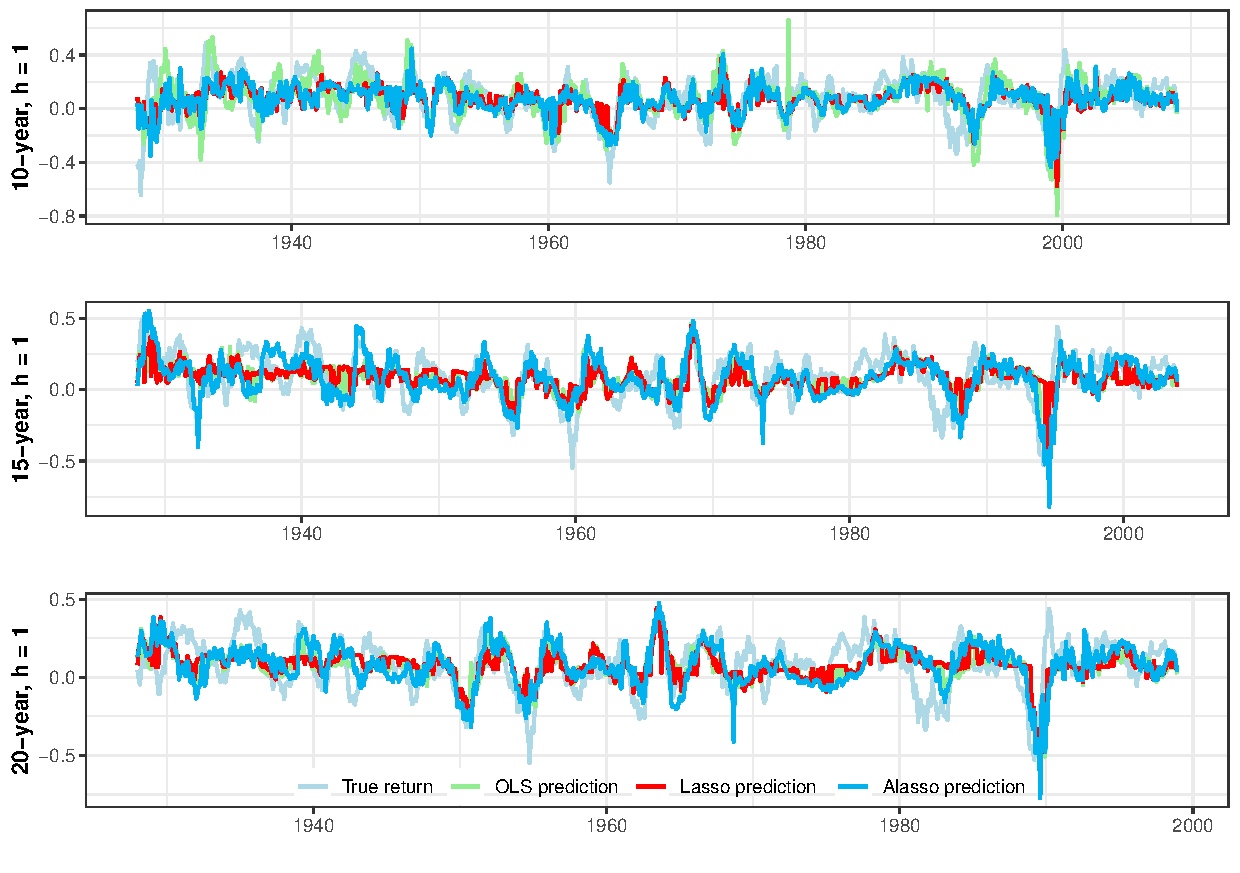
\includegraphics[scale = 0.695]{prediction_graph.pdf}
\end{center}
\end{figure}

Figure \ref{fig:2} shows how well predictions from OLS, alasso, and lasso estimators tracks true excess return. In general, from around 1950 to date, alasso and lasso estimators track true return quite well, and better the larger the sample size, though lagging behind true changes at some points. Alasso estimator adapts better to spikes while the path for lasso estimates is relatively 'smoother'. OLS estimator, on the other hand, adapts better to spikes for 10-year window, and gives more conservative estimates for 15- and 20-year window. All estimators are able to track the financial crisis, but do not follow the subsequent recovery very well except for alasso with 15-year estimation window. 

\begin{figure}
\begin{center}
		\caption{Estimated Coefficients (10-year rolling window $ (h = \frac{1}{12}) $)}
		\label{fig:3} 
		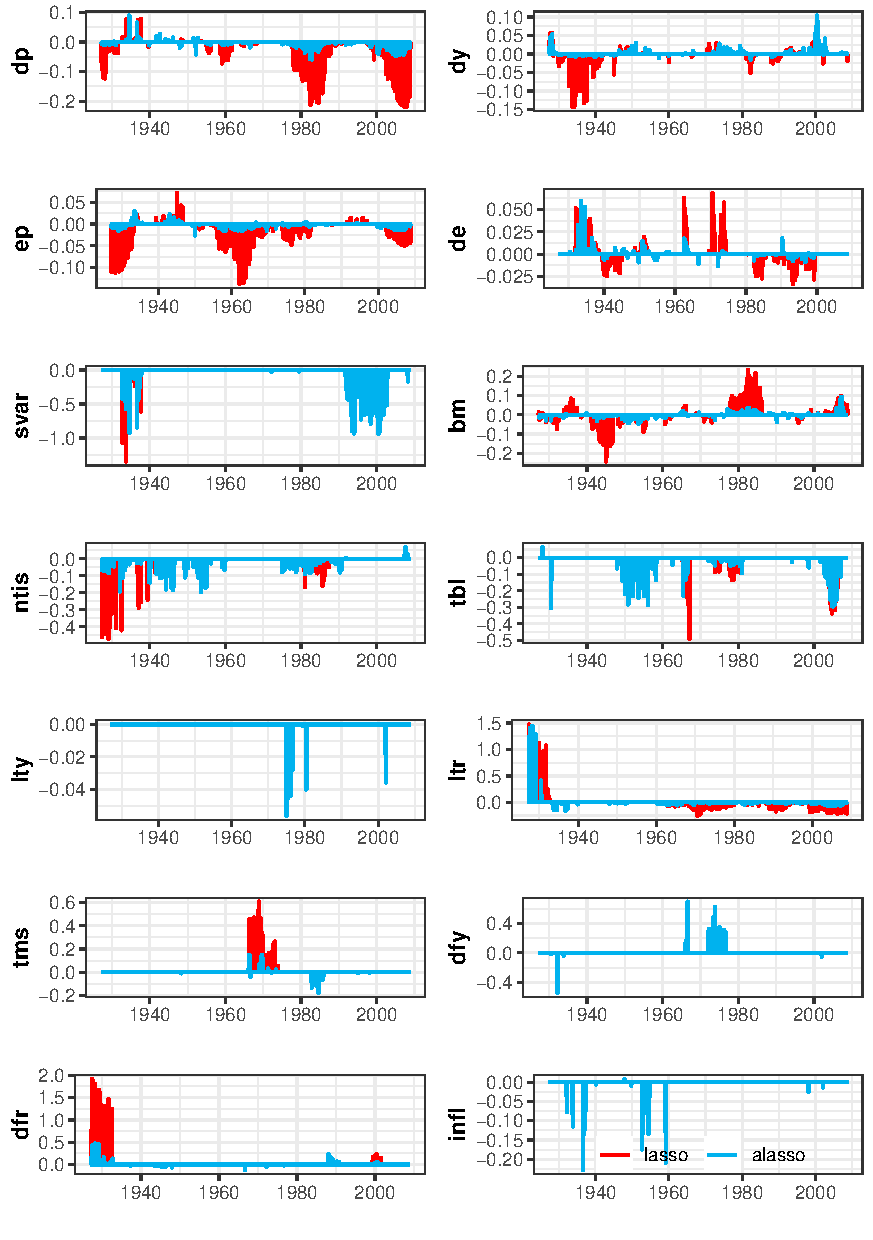
\includegraphics[scale = 0.96]{selection_graph_h1-2.pdf}
\end{center}
\end{figure}

Regarding screening, both shrinkage estimators select different predictors as estimation windows roll over. Some predictors are selected more frequently than others, and different rolling-windows call for different sets of predictors. The most frequently included predictors by alasso are \textbf{d/p}, \textbf{d/y}, \textbf{ntis}, \textbf{tbl}, and \textbf{ltr}. Some predictors even change sign as estimation windows roll over. These phenomena suggest the contribution of valuation ratios and macroeconomics predictors to excess return is dynamic over time. For example, inflation rate's estimated coefficients peak in between the 30s and 60s, coinciding with the period when the U.S experienced great fluctuation in inflation rate. Such high temporary variance may be reflected in the prices of stock market, giving the inflation rate higher contribution to excess return than in the periods of stability. In general, as alasso eliminates more predictors and estimates smaller coefficients, it thus leans toward smaller models that are more parsimonious \citep{lee2018lasso} with similar or in few cases better predictive performance than that of lasso and OLS. Illustrations for the case of 10-year rolling window and $ h = 1 $ are shown in Figure \ref{fig:4}.


\begin{figure}
\begin{center}
		\caption{Estimated Coefficients (10-year rolling window $ (h = 1) $)}
		\label{fig:4} 
		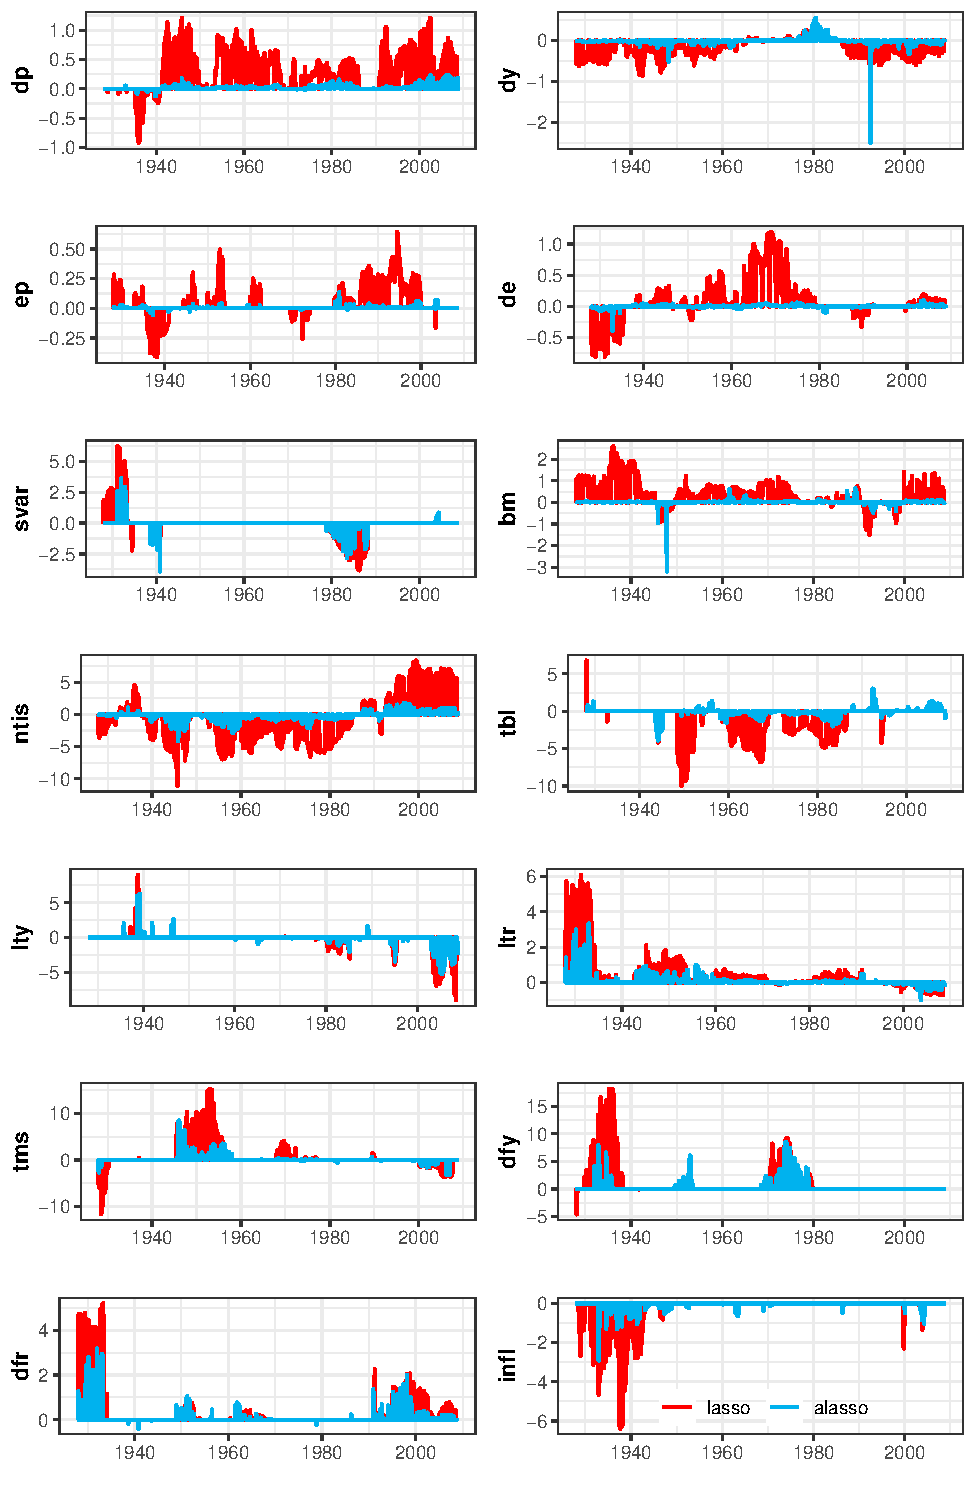
\includegraphics[scale = 0.88]{selection_graph.pdf}
\end{center}
\end{figure}

\section{Conclusion}

This paper discusses asymptotic theories and tests the performance of alasso and lasso estimator in context of two practical problems: mixed roots and near-singular design matrix. In order to achieve that goal, each problems are discussed at length, and an attempt to reconcile theories that address them are made. The theories are promising, especially for alasso: it has the ability to differentiate the true subset of variables even when the model contains a mix of I(0), I(1), and cointegrated processes thanks to an appropriate choices for the weights and tuning parameter $ \lambda $ while conventional lasso can only impose the restriction on I(0) processes if consistency is to be kept \citep{lee2018lasso}. Moreover, the tuning parameter for alasso can be further restricted to accommodate for near-singular design matrix, giving the estimator valid asymptotic distribution \citep{knight2008shrinkage}. Although the estimates are biased and convergence rate is less than optimal, it can correctly identify the true subset of variables as sample size grows.

Regarding the choice of tuning parameter, its growth rate plays a tremendous role in the performance of our shrinkage estimators. Generally, a slower-growing $ \lambda $ sequence emphasizes on picking out variables with true-large coefficients while sacrificing the success rate of identifying irrelevant ones; the opposite is true for a (relatively) faster-growing sequence. As all success rates slowly converge to 1, the 'best' choice of $ \lambda $ sequence lies in the hand of the user, who ultimately decides whether including or dropping variables yields more desirable outcome\footnote{Keep in mind that sample size for convergence may lie in the thousands. That is what mixed roots and near-singular design bring. However, in some field, this may not troublesome for much longer, as the amount of data is growing very fast}.
For starter, in this kind of complex predictive environment discussed here, I suggest $ \lambda_n = c_\lambda \frac{\sqrt{n}}{\log(n)^2} $ for alasso, and some $ \lambda_n $ that grow slower than $ \sqrt{n} $ for lasso.

Results for the empirical study are less than stellar. Our shrinkage estimators only occasionally perform better than OLS in terms of out-of-sample prediction error. Yet, looking past MPSE, alasso and lasso bring more to the table. The variable selection mechanism gives insight to the contribution of each predictors through time, as demonstrated in the inflation rate example above. Besides, more predictors can be included in the model, which may improve prediction accuracy.

For the complex nature of predictors presented in this paper, no exact post-selection inference for the discussed shrinkage estimators exists\footnote{or known to the author}. This is truly a serious drawback. Due to the incorporated variable selection mechanism, the reasonable thing to do is to pass ever more predictors into the model so that shrinkage estimators can pick out the better ones. As $ p $ increases, complications and complex interactions are bound to happen. Further research needs to be made so that a theory that can accommodate such scenario, increasing the practicality of shrinkage estimators.


\bibliographystyle{chicago}
\bibliography{thesis_bib}
\newpage
\section*{Affimation}

I hereby declare that I have composed my Master's thesis "LASSO-based predictive regression for stock returns" independently using only those resources mentioned, and that I have as such identified all passages which I have taken from publications verbatim or in substance. I agree that the work will be reviewed using plagiarism testing software.
\\~\\
Neither this thesis, nor any extract of it, has been previously submitted to an examining authority, in this or a similar form
\\~\\
I have ensured that the written version of this thesis is identical to the version saved on the enclosed storage medium.
\\[2in]
06.01.2019

\end{document}



 



